\documentclass[12pt,a4paper]{article}

\usepackage[a4paper,margin=1in]{geometry}
\usepackage{graphicx}
\usepackage{booktabs}
\usepackage{longtable}
\usepackage{array}
\usepackage{float}
\usepackage{hyperref}
\usepackage{xcolor}
\usepackage{caption}
\usepackage{subcaption}
\usepackage{listings}

\graphicspath{{figures/}}
\let\oldsection\section
\renewcommand{\section}{\clearpage\oldsection}
\lstset{
  basicstyle=\ttfamily\footnotesize,
  breaklines=true,
  frame=single,
  columns=fullflexible,
  showstringspaces=false,
  keepspaces=true
}

\title{\textbf{Large-Scale Huatuo Medical QA Processing and Comparative Analytics Using Hadoop Streaming and Apache Spark}}
\author{
Muammar Mohammed Abdullah Al-Ghrairi (24084470)\\
Muaz Been Amin (17221221)\\
WOC7017 Big Data Processing
}
\date{June 2026}

\begin{document}
\maketitle
\begin{center}
\textbf{Project Repository:} \url{https://github.com/Mr1-Robot/huatuo-big-data-hadoop-spark}
\end{center}

\begin{abstract}
This report presents the design, implementation, and evaluation of a big-data processing pipeline for the Huatuo medical question-answering datasets \cite{huatuo26m}. The project addresses a common challenge in healthcare data analytics: useful medical information is often distributed across heterogeneous sources with different schemas, different answer formats, and uneven metadata quality. Four Huatuo sources were therefore standardized into a canonical JSONL schema and unioned into a single analytical dataset while preserving source provenance. The final canonical dataset contains 34,048,898 records and occupies approximately 19 GB after enrichment with provenance, length, quality, hash, and duplicate metadata.

Four MapReduce-style case studies were developed and executed using Hadoop Streaming and Apache Spark on HDFS/YARN. The case studies analyse medical department demand, disease and symptom trends, medical QA quality and completeness, and question-type distribution. The work also includes a deterministic pilot stage, full-dataset inspection, data-flow diagrams, aggregation-technique documentation, and a controlled per-case-study benchmark. The full-dataset benchmark shows that Spark completed three of the four case studies faster, while Hadoop Streaming remained competitive for simple streaming text matching. The results demonstrate that framework performance depends not only on data size, but also on workload shape, startup overhead, aggregation complexity, and how much computation can benefit from Spark's execution model.
\end{abstract}

\section{Introduction}

Healthcare question-answering datasets contain valuable signals about patient concerns, disease mentions, medical departments, question intent, and answer quality. These signals can support exploratory public-health analytics, medical information retrieval, service-demand analysis, and dataset-quality assessment. However, large medical QA collections are rarely ready for direct distributed processing. They often combine multiple data sources, use inconsistent field names, mix textual and URL-based answers, contain repeated questions, and provide metadata only for selected subsets of the data. Before analytical algorithms can be applied, the data must therefore be inspected, standardized, cleaned, and transformed into a structure that can be processed consistently by big-data frameworks.

This project investigates how a large heterogeneous medical QA collection can be prepared for distributed analytics and processed using two big-data frameworks: Hadoop Streaming \cite{hadoop} and Apache Spark \cite{spark}. The selected Huatuo sources are suitable for this task because together they exceed the project size requirement and represent realistic integration issues: the sources share a medical QA theme, but they do not share a reliable global key that would justify joining them. For this reason, the project uses schema normalization followed by union. This keeps each original record as an independent observation while preserving provenance through source-related fields.

The analytical work is organized into four case studies. The department-demand case study aggregates records by medical department to show which departments are most represented in the available metadata. The disease and symptom trend case study performs rule-based text scanning and term aggregation to identify frequent medical mentions. The QA quality and completeness case study measures source-level reliability through missing-value counts, URL/text answer classification, duplicate flags, text-length statistics, and quality scores where available. The question-type distribution case study classifies questions into intent categories such as treatment, diagnosis, symptoms, medication, prevention, cause, and other.

The implementation follows a MapReduce view of data processing. Each case study maps canonical JSONL records into analytical key-value pairs, groups records by a case-specific key, and reduces each group into counts or summary statistics. Equivalent implementations were prepared for Hadoop Streaming and PySpark so that both frameworks processed the same canonical input and produced comparable outputs. A deterministic 400,000-record pilot was used to validate the pipeline before running the full 34-million-record dataset on HDFS/YARN.

The remainder of this report describes the dataset, integration method, canonical schema, preprocessing decisions, full dataset inspection, analytics lifecycle, MapReduce data-flow diagrams, aggregation techniques, experimental setup, benchmark results, and limitations. This structure follows the project guideline requirement to document both the big-data analytics lifecycle and the data-flow design of the developed MapReduce algorithms.

\section{Dataset Description}

The project uses four Huatuo sources. The original source snapshot contains 34,048,913 records and 5.432 GB of JSONL data. Table~\ref{tab:dataset-sources} summarizes the input sources.

\begin{table}[H]
\centering
\caption{Huatuo source datasets}
\label{tab:dataset-sources}
\begin{tabular}{lrrl}
\toprule
Source & Records & Size & Main fields \\
\midrule
Consultation QA & 32,708,346 & 4.537 GB & questions, answers \\
Encyclopedia QA & 364,420 & 0.608 GB & questions, answers \\
Knowledge Graph QA & 798,444 & 0.149 GB & questions, answers \\
Huatuo26M-Lite & 177,703 & 0.138 GB & id, question, answer, score, label \\
\bottomrule
\end{tabular}
\end{table}

\begin{figure}[H]
\centering

\includegraphics[width=0.92\linewidth]{source_distribution.png}
\caption{Source distribution in the full canonical dataset. A logarithmic scale is used because Consultation QA dominates the record count.}
\end{figure}

\section{Data Integration Method}

The Huatuo sources were integrated using schema normalization and union rather than joins. A join would require a trustworthy shared key such as a patient identifier, consultation identifier, or universal question identifier. Such a key is not available across the sources. The datasets share the same broad domain, medical question answering, but each row represents an independent QA observation rather than a guaranteed reference to the same patient, consultation, disease event, or medical encounter. Joining records would therefore create unsupported relationships between different medical QA records.

The integration strategy was therefore:

\begin{enumerate}
\item Read each original source file independently.
\item Convert each raw record into one canonical medical QA record.
\item Preserve source provenance instead of merging unrelated records.
\item Append all canonical records into one unified JSONL file.
\item Mark duplicate questions across the complete union using a stable question hash.
\end{enumerate}

This approach is a union, not a relational join. It keeps the analytical meaning of the data clear: every output row is one normalized QA observation, and the \texttt{source} and \texttt{source\_split} fields explain where that observation came from.

\subsection{Source Field Alignment}

The four sources used different field names for similar concepts. The standardization script used field aliases to select the first available value for each canonical concept. Table~\ref{tab:field-alignment} summarizes the main mapping.

\begin{table}[H]
\centering
\small
\caption{Field alignment from heterogeneous Huatuo records to the canonical schema}
\label{tab:field-alignment}
\begin{tabular}{p{0.25\linewidth}p{0.34\linewidth}p{0.31\linewidth}}
\toprule
Canonical concept & Accepted raw aliases & Normalized output field \\
\midrule
Record identifier & \texttt{record\_id}, \texttt{id}, \texttt{ID}, \texttt{\_id} & \texttt{record\_id} \\
Question text & question aliases including plural and sequence forms & \texttt{question} \\
Answer content & answer aliases including plural and sequence forms & \texttt{answer} \\
Quality score & \texttt{quality\_score}, \texttt{score}, \texttt{Expert\_Score} & \texttt{quality\_score} \\
Department label & \texttt{department}, \texttt{label}, \texttt{Department\_Label} & \texttt{department} \\
Related disease & \texttt{related\_disease}, \texttt{related\_diseases}, \texttt{Related\_Diseases}, \texttt{disease} & \texttt{related\_disease} \\
\bottomrule
\end{tabular}
\end{table}

For example, Consultation QA stores its content using plural fields such as \texttt{questions} and \texttt{answers}, while Huatuo26M-Lite uses direct fields such as \texttt{id}, \texttt{question}, \texttt{answer}, \texttt{score}, \texttt{label}, and \texttt{related\_diseases}. The alias-based mapping allowed both layouts to produce the same canonical fields without writing a separate analytical program for each source.

\subsection{Text Normalization}

The normalization step was intentionally conservative. The medical text was not translated, rewritten, summarized, corrected, or clinically interpreted. Normalization only made the data technically consistent for distributed processing. The exact text-handling rules were:

\begin{itemize}
\item Null values were converted to empty strings during processing and later represented as null where the canonical field was optional.
\item List-valued fields were joined into one string with spaces. This was necessary because some sources store question or answer text as a list.
\item Dictionary-valued fields were serialized into deterministic JSON text using sorted keys.
\item Repeated whitespace was collapsed into a single space.
\item Leading and trailing whitespace was stripped.
\item Question hashing used the normalized question after case folding.
\end{itemize}

Table~\ref{tab:normalization-examples} shows representative examples of how raw values were standardized.

\begin{table}[H]
\centering
\small
\caption{Examples of normalization decisions}
\label{tab:normalization-examples}
\begin{tabular}{p{0.28\linewidth}p{0.30\linewidth}p{0.32\linewidth}}
\toprule
Raw situation & Normalization action & Reason \\
\midrule
\texttt{questions} contains a one-item list & Join list items into one \texttt{question} string & Allows all sources to use the same text field \\
\texttt{answers} starts with \texttt{https://} & Mark as URL answer and set answer length to 0 & URL answers are links, not answer text for length analysis \\
Lite record has \texttt{score=5} & Convert score to numeric quality score & Enables average, minimum, and maximum score aggregation \\
Lite record has \texttt{label} & Store label as department; mark metadata as observed & Department metadata came directly from the source \\
Source has no department or disease field & Store optional metadata as null; mark metadata as unavailable & Avoids inventing metadata when it is not observed \\
Repeated or differently cased question text & Hash normalized, casefolded question text & Enables duplicate detection across the full union \\
\bottomrule
\end{tabular}
\end{table}

\subsection{Canonical Record Construction}

After field alignment and text normalization, each raw row was converted into a canonical JSONL object. The main generated fields were:

\begin{itemize}
\item \texttt{answer\_type}: classified as \texttt{url}, \texttt{text}, or \texttt{empty}.
\item \texttt{metadata\_origin}: classified as \texttt{observed}, \texttt{inferred}, or \texttt{unavailable}. In the final full summary, observed metadata came from Huatuo26M-Lite and unavailable metadata came from sources without department or disease fields.
\item \texttt{question\_length}: number of characters in the normalized question.
\item \texttt{answer\_length}: number of characters in the normalized answer when the answer is text; URL answers use 0.
\item \texttt{question\_hash}: SHA-256 hash of the normalized, casefolded question.
\item \texttt{duplicate\_flag}: Boolean flag set during the full union when the same question hash had already appeared.
\end{itemize}

When a raw record did not provide a stable identifier, the pipeline generated one using the source name, source split, row number, and the first characters of the question hash. This made records traceable without assuming a global source identifier existed.

\subsection{Transformation Examples}

Table~\ref{tab:source-transform-examples} shows how two representative source layouts become canonical analytical records.

\begin{table}[H]
\centering
\small
\caption{Representative source-to-canonical transformations}
\label{tab:source-transform-examples}
\begin{tabular}{p{0.22\linewidth}p{0.33\linewidth}p{0.35\linewidth}}
\toprule
Source type & Raw structure & Canonical result \\
\midrule
Consultation QA & Question list plus URL answer list & Consultation source, train split, normalized question, URL answer, no observed department or disease, unavailable metadata \\
Huatuo26M-Lite & ID, question, answer, score, label, and related disease fields & Lite source, full split, text answer, numeric quality score, observed department, optional observed disease, observed metadata \\
Encyclopedia QA and Knowledge Graph QA & Medical question and text answer fields with source-specific names & Source-specific provenance, normalized question, text answer, derived text lengths, and duplicate hash \\
\bottomrule
\end{tabular}
\end{table}

A simplified canonical record has the following structure:

\begin{verbatim}
{
  "record_id": "consultation-train-1-34890e61cc97",
  "source": "consultation",
  "source_split": "train",
  "question": "Normalized medical question text",
  "answer": "https://www.example.org/question/detail/...",
  "answer_type": "url",
  "department": null,
  "related_disease": null,
  "quality_score": null,
  "metadata_origin": "unavailable",
  "question_length": 28,
  "answer_length": 0,
  "question_hash": "sha256-value",
  "duplicate_flag": false
}
\end{verbatim}

\subsection{Duplicate Detection Across the Union}

Duplicate detection was performed after source-level standardization, during the full union step. The pipeline used a SQLite database containing one table of previously seen question hashes. For each canonical record, the union script attempted to insert its \texttt{question\_hash}. If the insertion succeeded, the record was treated as the first occurrence. If the insertion failed because the hash already existed, the record was marked with \texttt{duplicate\_flag=true}. The record was still kept in the final dataset because the objective was analytical union with duplicate visibility, not duplicate removal.

This design has two benefits. First, it scales better than keeping all 34 million hashes only in Python memory during the full union. Second, it preserves duplicate records for later quality analysis. The full canonical dataset therefore records both the original QA observations and whether each question had appeared before.

\section{Canonical Schema, Preprocessing, and Pilot Validation}

After the integration method was defined, the next stage was to create a stable preprocessing pipeline that could produce the same analytical input for both Hadoop Streaming and Spark. This stage was important because the objective of the project was not only to run four case studies, but to ensure that both frameworks processed the same records, the same fields, and the same derived values.

\subsection{Canonical Schema Design}

Each source record was transformed into a canonical JSONL record. JSONL was selected because it is line-oriented, streamable, compatible with Hadoop Streaming, and easy for Spark to read as semi-structured data. The schema stores five groups of fields:

\begin{itemize}
\item Identity and provenance fields store the record ID, source name, and source split.
\item Medical QA content fields store the question, answer, answer type, department, and related disease.
\item Quality fields store quality score and metadata origin.
\item Measurement fields store question length and answer length.
\item Deduplication fields store the normalized question hash and duplicate flag.
\end{itemize}

Table~\ref{tab:canonical-schema} explains the main canonical fields and why each field was needed.

\begin{table}[H]
\centering
\small
\caption{Canonical schema fields used by the analytical pipeline}
\label{tab:canonical-schema}
\begin{tabular}{p{0.25\linewidth}p{0.21\linewidth}p{0.44\linewidth}}
\toprule
Field & Type & Purpose \\
\midrule
\texttt{record\_id} & string & Stable row identifier from the source or generated from source, split, row number, and question hash \\
\texttt{source} & string & Identifies the originating dataset: consultation, encyclopedia, knowledge graph, or lite \\
\texttt{source\_split} & string & Preserves train, validation, test, or full split information \\
\texttt{question} & string & Normalized medical question text used by all case studies \\
\texttt{answer} & string & Normalized answer text or URL \\
\texttt{answer\_type} & category & Separates text answers from URL answers and empty answers \\
\texttt{department} & nullable string & Observed department label where the source provides it \\
\texttt{related\_disease} & nullable string & Observed related disease where the source provides it \\
\texttt{quality\_score} & nullable number & Numeric quality score, available mainly in Huatuo26M-Lite \\
\texttt{metadata\_origin} & category & Indicates whether metadata was observed, inferred, or unavailable \\
\texttt{question\_length} & integer & Character length of the normalized question \\
\texttt{answer\_length} & integer & Character length of text answers; URL answers use 0 \\
\texttt{question\_hash} & string & SHA-256 hash used for duplicate detection \\
\texttt{duplicate\_flag} & Boolean & Marks repeated questions across the full union \\
\bottomrule
\end{tabular}
\end{table}

\subsection{Preprocessing Operations}

The preprocessing stage consisted of deterministic operations that could be repeated from the source snapshots. Question normalization was limited to formatting cleanup. It did not translate, rewrite, summarize, or medically correct question text. The process handled missing values, joined list-valued fields, converted dictionary-valued fields into JSON text, collapsed repeated whitespace, and stripped leading or trailing spaces. Duplicate detection used a casefolded normalized question and SHA-256 hashing.

The preprocessing operations can be summarized as follows:

\begin{enumerate}
\item Parse each JSON or JSONL source file and reject invalid non-object records.
\item Select source fields using the alias rules described in Section 3.
\item Normalize question and answer values into single strings.
\item Classify each answer as URL, text, or empty.
\item Convert available quality scores into numeric values.
\item Preserve observed department and disease metadata where available.
\item Generate missing record identifiers where the source does not provide one.
\item Compute question and answer lengths.
\item Compute the SHA-256 question hash.
\item Write standardized records as canonical JSONL.
\item Union all canonical JSONL files and mark duplicate questions.
\end{enumerate}

The output of this stage was the canonical dataset used by both frameworks. Hadoop read the same JSONL lines through streaming mapper programs, while Spark read the same JSONL records through PySpark. This avoided a common benchmark problem where two frameworks are compared using different preprocessing assumptions.

\subsection{Pilot Dataset Construction}

Before processing the full dataset, a deterministic pilot dataset was created. The pilot contained 400,000 canonical records: 100,000 from each of the four sources. The purpose of the pilot was to validate the schema, run all four analytical case studies end to end, confirm that Hadoop and Spark produced equivalent aggregate outputs, and expose runtime or formatting problems before the full 34-million-record run.

\begin{table}[H]
\centering
\caption{Pilot dataset composition}
\label{tab:pilot-composition}
\begin{tabular}{lr}
\toprule
Pilot component & Records \\
\midrule
Consultation QA & 100,000 \\
Encyclopedia QA & 100,000 \\
Knowledge Graph QA & 100,000 \\
Huatuo26M-Lite & 100,000 \\
\midrule
Total pilot records & 400,000 \\
\bottomrule
\end{tabular}
\end{table}

The pilot preserved the source-split structure where available. For Consultation QA, Encyclopedia QA, and Knowledge Graph QA, the pilot used 98,000 training records, 1,000 validation records, and 1,000 test records from each source. Huatuo26M-Lite was represented as a full split with 100,000 records. This gave a balanced pilot across sources while still including train, validation, and test records.

\subsection{Pilot Inspection Results}

The pilot inspection confirmed that the canonical schema was usable before full-scale execution. Table~\ref{tab:pilot-summary} summarizes the pilot inspection results.

\begin{table}[H]
\centering
\caption{Pilot canonical dataset inspection}
\label{tab:pilot-summary}
\begin{tabular}{lr}
\toprule
Metric & Value \\
\midrule
Pilot records & 400,000 \\
Text answers & 300,000 \\
URL answers & 100,000 \\
Observed metadata records & 100,000 \\
Unavailable metadata records & 300,000 \\
Duplicate-flagged records & 709 \\
Duplicate percentage & 0.1772\% \\
\bottomrule
\end{tabular}
\end{table}

These values were useful for validating the pipeline. The 100,000 URL answers came from the Consultation QA pilot records, while the text answers came from the other three sources. The 100,000 observed metadata records came from Huatuo26M-Lite, which provides department and quality metadata. The low duplicate percentage in the pilot also confirmed that duplicate detection was functioning without unexpectedly collapsing the dataset.

\subsection{Pilot Case-Study Validation}

After the pilot dataset was inspected, all four case studies were executed on HDFS/YARN using both Hadoop Streaming and Spark. The pilot was not used as the final performance conclusion; it was used to confirm execution correctness, output structure, and framework equivalence before the full dataset run.

\begin{table}[H]
\centering
\caption{Pilot HDFS/YARN benchmark and output validation}
\label{tab:pilot-benchmark}
\begin{tabular}{lrrr}
\toprule
Case study & Output groups & Hadoop & Spark \\
\midrule
Department demand & 16 & 18.763 s & 29.630 s \\
Disease and symptom trends & 2,301 & 18.558 s & 31.256 s \\
QA quality and completeness & 4 & 19.602 s & 25.309 s \\
Question-type distribution & 7 & 18.560 s & 23.310 s \\
\bottomrule
\end{tabular}
\end{table}

The output group counts in Table~\ref{tab:pilot-benchmark} show that each framework generated the same number of analytical groups for every case study. This was a key validation point because it showed that the Hadoop mapper/reducer pipeline and the Spark application were applying equivalent grouping logic to the same canonical input.

The pilot timing pattern also helped explain later results. Spark was slower than Hadoop in the pilot because the workload was small relative to Spark startup, session creation, scheduling, and execution-planning overhead. This did not mean Spark was unsuitable for the project; it meant the pilot was mainly a correctness and readiness test. The full dataset benchmark in Section 10 provides the more meaningful performance comparison.

\subsection{Pilot Analytical Observations}

The pilot produced several early analytical observations that were later checked at full scale:

\begin{itemize}
\item The Consultation QA pilot records used URL answers, which required answer-type classification before answer-length analysis.
\item Huatuo26M-Lite provided observed metadata such as department labels and quality scores, making it important for department-demand and quality analysis.
\item Disease and symptom trend mining generated many more output groups than the other case studies because it searched for medical terms and grouped by matched term.
\item QA quality and completeness produced only four output groups because it aggregated at source level.
\item Question-type distribution produced seven output groups because the rule-based classifier used seven intent categories.
\end{itemize}

The pilot stage therefore served as a controlled rehearsal for the full project. It verified that the canonical schema, preprocessing logic, Hadoop jobs, Spark jobs, output paths, and benchmark logging were ready before the 19 GB canonical dataset was submitted to HDFS/YARN.

\section{Final Dataset Inspection and Readiness}

After schema normalization, preprocessing, pilot validation, and full union, the project produced one final canonical dataset for distributed processing. This section focuses only on that completed dataset and the checks used to confirm that it was ready for Hadoop Streaming and Spark.

The final dataset path in the project workspace was:

\begin{verbatim}
data/standardized-full/huatuo_unified.jsonl
\end{verbatim}

The file was later uploaded to HDFS as the shared full benchmark input:

\begin{verbatim}
/healthcare/full/input/huatuo_unified.jsonl
\end{verbatim}

The final canonical dataset contains 34,048,898 records. The original source snapshot contained 34,048,913 records, so 15 source records were not retained because they did not provide usable question text after normalization. This is a small removal relative to the full dataset and ensured that every final row had a valid analytical question field.

The final canonical file is larger than the raw source snapshot. The raw source data was approximately 5.432 GB, while the final canonical JSONL file was approximately 19 GB. This increase is expected because every row was enriched with explicit provenance, answer type, metadata origin, quality fields, text-length fields, question hash, and duplicate flag. The larger file is therefore not duplicated storage by accident; it is the analytical representation required for consistent Hadoop and Spark processing.

\begin{table}[H]
\centering
\caption{Final canonical dataset summary}
\label{tab:full-summary}
\begin{tabular}{lr}
\toprule
Metric & Value \\
\midrule
Final canonical records & 34,048,898 \\
Original source records & 34,048,913 \\
Records excluded after normalization & 15 \\
Final canonical file size & 20,168,846,076 bytes, about 19 GB \\
Invalid JSON lines & 0 \\
Missing questions & 0 \\
Missing answers & 0 \\
\bottomrule
\end{tabular}
\end{table}

\subsection{Final Source Composition}

Table~\ref{tab:full-source-composition} shows the final source composition after standardization and union. Consultation QA dominates the full dataset, while Huatuo26M-Lite is smaller but important because it contributes observed department and quality metadata.

\begin{table}[H]
\centering
\caption{Final canonical records by source}
\label{tab:full-source-composition}
\begin{tabular}{lr}
\toprule
Source & Records \\
\midrule
Consultation QA & 32,708,331 \\
Knowledge Graph QA & 798,444 \\
Encyclopedia QA & 364,420 \\
Huatuo26M-Lite & 177,703 \\
\midrule
Total & 34,048,898 \\
\bottomrule
\end{tabular}
\end{table}

The split distribution was also preserved. Consultation QA contributed 32,706,331 training records, 1,000 validation records, and 1,000 test records. Encyclopedia QA contributed 362,420 training records plus 1,000 validation and 1,000 test records. Knowledge Graph QA contributed 796,444 training records plus 1,000 validation and 1,000 test records. Huatuo26M-Lite was represented as a full split with 177,703 records. This split preservation is useful because it keeps the dataset traceable even though the project analytics process the union as one canonical file.

\subsection{Answer-Type and Metadata Readiness}

The final dataset contains both URL answers and text answers. This distinction mattered because Consultation QA mostly contains answer URLs, while the other sources contain answer text. The preprocessing stage therefore classified every answer before the analytical stage.

\begin{table}[H]
\centering
\caption{Final answer and metadata classification}
\label{tab:full-answer-metadata}
\begin{tabular}{lr}
\toprule
Metric & Records \\
\midrule
URL answers & 32,708,326 \\
Text answers & 1,340,572 \\
Observed metadata & 177,703 \\
Unavailable metadata & 33,871,195 \\
\bottomrule
\end{tabular}
\end{table}

The answer-type split shaped the interpretation of later results. URL answers were valid answers, but they were not treated as answer text for length analysis. Therefore, URL answer records were assigned an answer length of 0. This explains why the overall average answer length in the full dataset is low even though the text-answer sources contain long medical answers.

\subsection{Duplicate and Quality Readiness}

Duplicate handling was performed by flagging repeated normalized question hashes. Duplicates were not removed because the final dataset needed to preserve the full source evidence while still exposing repetition for quality analysis.

\begin{table}[H]
\centering
\caption{Final duplicate and quality indicators}
\label{tab:full-quality}
\begin{tabular}{lr}
\toprule
Metric & Value \\
\midrule
Duplicate-flagged records & 10,162,575 \\
Duplicate percentage & 29.847\% \\
Quality-score records & 177,703 \\
Average quality score & 4.1281 \\
Minimum quality score & 4.0 \\
Maximum quality score & 5.0 \\
\bottomrule
\end{tabular}
\end{table}

The duplicate percentage is important for the report because it shows that the pipeline did more than count records. It created a dataset-quality signal that could be used by the QA quality and completeness case study. The quality-score values come from Huatuo26M-Lite and were converted to numeric form during preprocessing, which made average, minimum, and maximum aggregation possible.

\subsection{Text-Length Readiness}

Text lengths were precomputed so that both Hadoop and Spark could aggregate the same values without each framework making different assumptions about how to measure text. Table~\ref{tab:full-lengths} summarizes the final length statistics.

\begin{table}[H]
\centering
\caption{Final question and answer length statistics}
\label{tab:full-lengths}
\begin{tabular}{lrrr}
\toprule
Field & Minimum & Average & Maximum \\
\midrule
Question length & 1 & 17.4845 & 428 \\
Answer length & 0 & 7.3764 & 43,809 \\
\bottomrule
\end{tabular}
\end{table}

The answer maximum shows that some text answers are long, while the answer average is low because URL answers use length 0. This design allowed the quality case study to distinguish source behavior rather than mixing URL strings with medical answer text.

\subsection{Department Metadata in the Final Dataset}

Observed department metadata was available mainly from Huatuo26M-Lite. Figure~\ref{fig:top-departments} summarizes the top observed departments after standardization. This metadata was used directly by the medical department demand case study.

\begin{figure}[H]
\centering

\includegraphics[width=0.92\linewidth]{top_departments.png}
\caption{Top observed departments in the final canonical dataset.}
\label{fig:top-departments}
\end{figure}

\begin{figure}[H]
\centering
\begin{subfigure}{0.47\linewidth}
\centering

\includegraphics[width=\linewidth]{answer_type_distribution.png}
\caption{Answer type distribution}
\end{subfigure}
\hfill
\begin{subfigure}{0.47\linewidth}
\centering

\includegraphics[width=\linewidth]{duplicate_records.png}
\caption{Duplicate-flagged records}
\end{subfigure}
\caption{Full dataset inspection figures generated from \texttt{reports/full\_summary.json}.}
\end{figure}

\subsection{Readiness Checklist}

The final dataset was considered ready for distributed analytics because it satisfied the following conditions:

\begin{itemize}
\item It was a single line-oriented JSONL file that could be streamed by Hadoop and read by Spark.
\item Every record had a non-empty normalized question.
\item Every record had an answer field classified as URL or text.
\item Invalid JSON line count was 0.
\item Missing question count was 0.
\item Missing answer count was 0.
\item Source provenance was preserved for every row.
\item Duplicate status was available through \texttt{duplicate\_flag}.
\item Length, quality, answer type, and metadata-origin fields were precomputed consistently.
\item The same final file was used as the input for all full Hadoop and Spark case-study jobs.
\end{itemize}

At this point the dataset was no longer a set of heterogeneous source files. It was a prepared analytical dataset with stable schema, validated structure, preserved provenance, duplicate visibility, and derived fields required by the four case studies.

\section{Big Data Analytics Lifecycle Mapping}

The project guideline requires the report to describe the Big Data Analytics Lifecycle stages. In this project, the lifecycle was not treated as a theoretical list. Each stage corresponded to a concrete activity, script output, dataset artifact, benchmark result, or report figure. Table~\ref{tab:lifecycle-mapping} maps the lifecycle stages to the work completed in this project.

\begin{table}[H]
\centering
\small
\caption{Mapping of Big Data Analytics Lifecycle stages to the project work}
\label{tab:lifecycle-mapping}
\begin{tabular}{p{0.22\linewidth}p{0.39\linewidth}p{0.29\linewidth}}
\toprule
Lifecycle stage & What was done in this project & Evidence or output \\
\midrule
Data generation & Selected the Huatuo medical question-answering sources as the raw data domain & Four Huatuo source datasets \\
Data acquisition & Obtained the source snapshots and inspected their raw sizes and record counts & Original sources: 34,048,913 records, 5.432 GB \\
Data aggregation & Placed all source files under one project workflow so they could be processed consistently & Unified preprocessing workspace \\
Data preprocessing & Parsed JSON/JSONL records, aligned field aliases, normalized text formatting, classified answers, and generated derived fields & Canonical JSONL records \\
Data integration & Used schema normalization and union rather than joins because no reliable shared global key existed & Final unified dataset \\
Data cleaning & Checked invalid JSON, missing questions, missing answers, answer type, metadata availability, and duplicate hashes & 0 invalid JSON lines, 0 missing questions, 0 missing answers \\
Data reduction & Created a deterministic 400,000-record pilot dataset before full execution & Balanced pilot with 100,000 records per source \\
Data transformation & Produced the final line-oriented analytical dataset for Hadoop and Spark & 19 GB canonical JSONL file \\
Data analytics & Implemented four MapReduce-style case studies over the canonical dataset & Department, term trend, QA quality, and question-type outputs \\
Evaluation & Ran equivalent Hadoop Streaming and Spark jobs on HDFS/YARN & Pilot and full benchmark tables and charts \\
Reporting & Converted evidence into tables, figures, DFDs, and discussion & Final report and generated figures \\
\bottomrule
\end{tabular}
\end{table}

This mapping shows that the lifecycle was followed end to end. The early stages prepared a trustworthy analytical dataset, the middle stages validated and transformed it, and the later stages used distributed processing to answer the four case-study questions. The lifecycle also explains why the project did not move directly from raw data to benchmarking: without schema alignment, validation, pilot testing, and final readiness checks, the Hadoop and Spark results would not have been comparable.

\section{MapReduce Case Studies and Data Flow Diagrams}

The four case studies were implemented twice: once using Hadoop Streaming mapper/reducer programs and once using PySpark DataFrame transformations. Both versions read the same canonical JSONL input and wrote JSON output groups. The difference is the processing model. Hadoop Streaming explicitly emits key-value pairs, sorts and groups them through the Hadoop shuffle, and reduces each grouped key. Spark expresses the same logic through DataFrame operations such as selection, user-defined functions, explosion of arrays, grouping, aggregation, ordering, and JSON writing.

\subsection{Case Study 1: Medical Department Demand}

This case study measures observed and inferred medical department demand. It mainly uses the \texttt{department} field from Huatuo26M-Lite, and it can also infer departments from disease terms when department metadata is unavailable. The grouping key is department plus metadata origin.

\subsubsection*{Hadoop Streaming Implementation}

The Hadoop mapper reads one canonical JSONL record at a time. If a department is available, it emits a department key with value 1. If no department is available, the mapper checks disease terms from the analytics rules and emits inferred department keys where possible. The Hadoop shuffle groups identical department-origin keys. The reducer sums the values for each key and outputs department demand counts.

\begin{figure}[H]
\centering
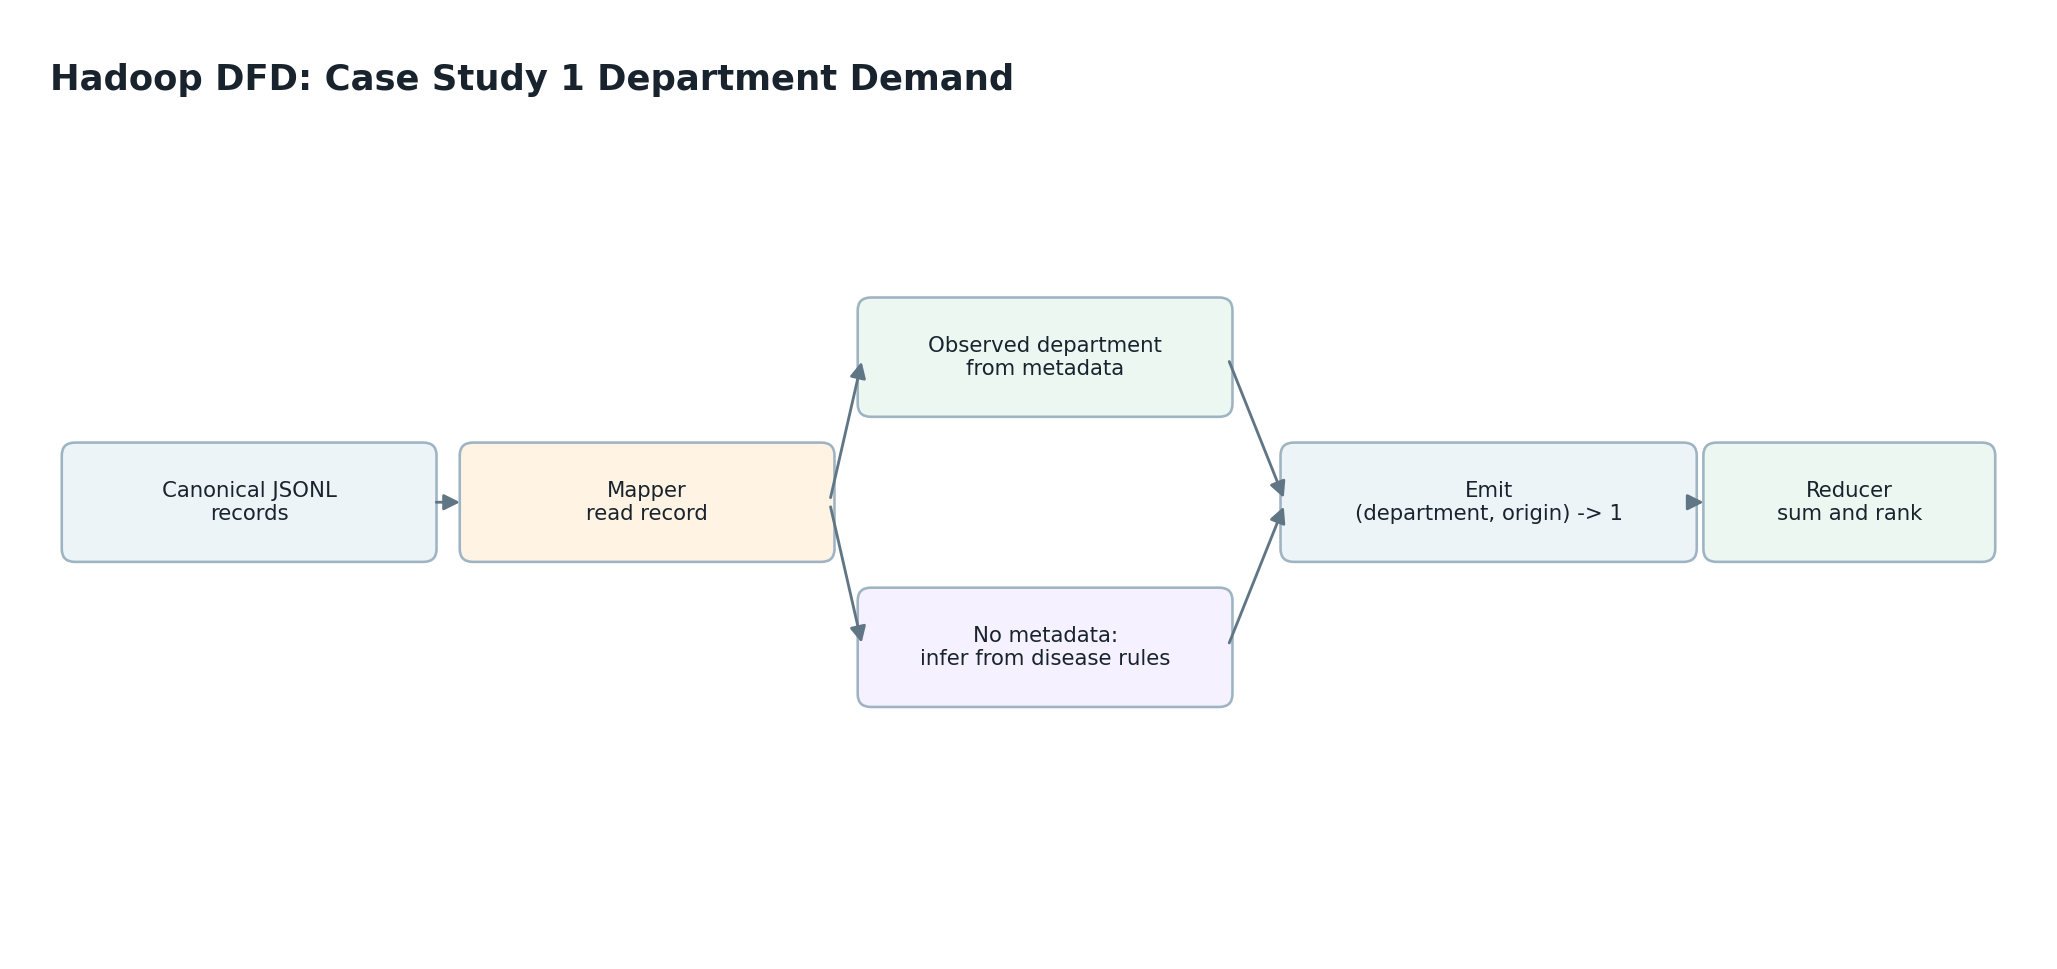
\includegraphics[width=\linewidth]{dfd_case_study_1_department_demand.png}
\caption{Hadoop Streaming data flow for Case Study 1: Medical Department Demand.}
\end{figure}

The DFD above can be read as a MapReduce key construction process. The input data store is the canonical JSONL file in HDFS. Each mapper receives independent records and extracts \texttt{department}, \texttt{inferred\_department}, and \texttt{question}. The mapper does not output the full record. It outputs a compact analytical key that represents the department bucket and a numeric value that represents one record contributing to that bucket. Hadoop then performs the shuffle and sort phase, which is not a simple file copy: it physically groups all identical department keys before they reach the reducer. The reducer receives one department-origin group at a time and adds the integer values to create the final department demand count.

\begin{table}[H]
\centering
\caption{Case Study 1 Hadoop key-value design}
\label{tab:cs1-hadoop-kv}
\begin{tabular}{p{0.26\linewidth}p{0.62\linewidth}}
\toprule
Element & Meaning \\
\midrule
Input fields & \texttt{department}, \texttt{inferred\_department}, \texttt{question} \\
Mapper key & \texttt{["department", department, origin]} \\
Mapper value & \texttt{1}, meaning one record belongs to that department-origin bucket \\
Shuffle key & Exact JSON key string, so all identical department-origin groups are placed together \\
Reducer output & \texttt{\{"key": [...], "metrics": \{"count": total\}\}} \\
\bottomrule
\end{tabular}
\end{table}

\subsubsection*{Spark Implementation}

The Spark job reads the canonical JSONL file into a DataFrame. It selects observed departments where they exist, applies an inference function for records without department metadata, unions observed and inferred department rows, groups by department and origin, counts records, orders the result, and writes JSON output.

\begin{figure}[H]
\centering
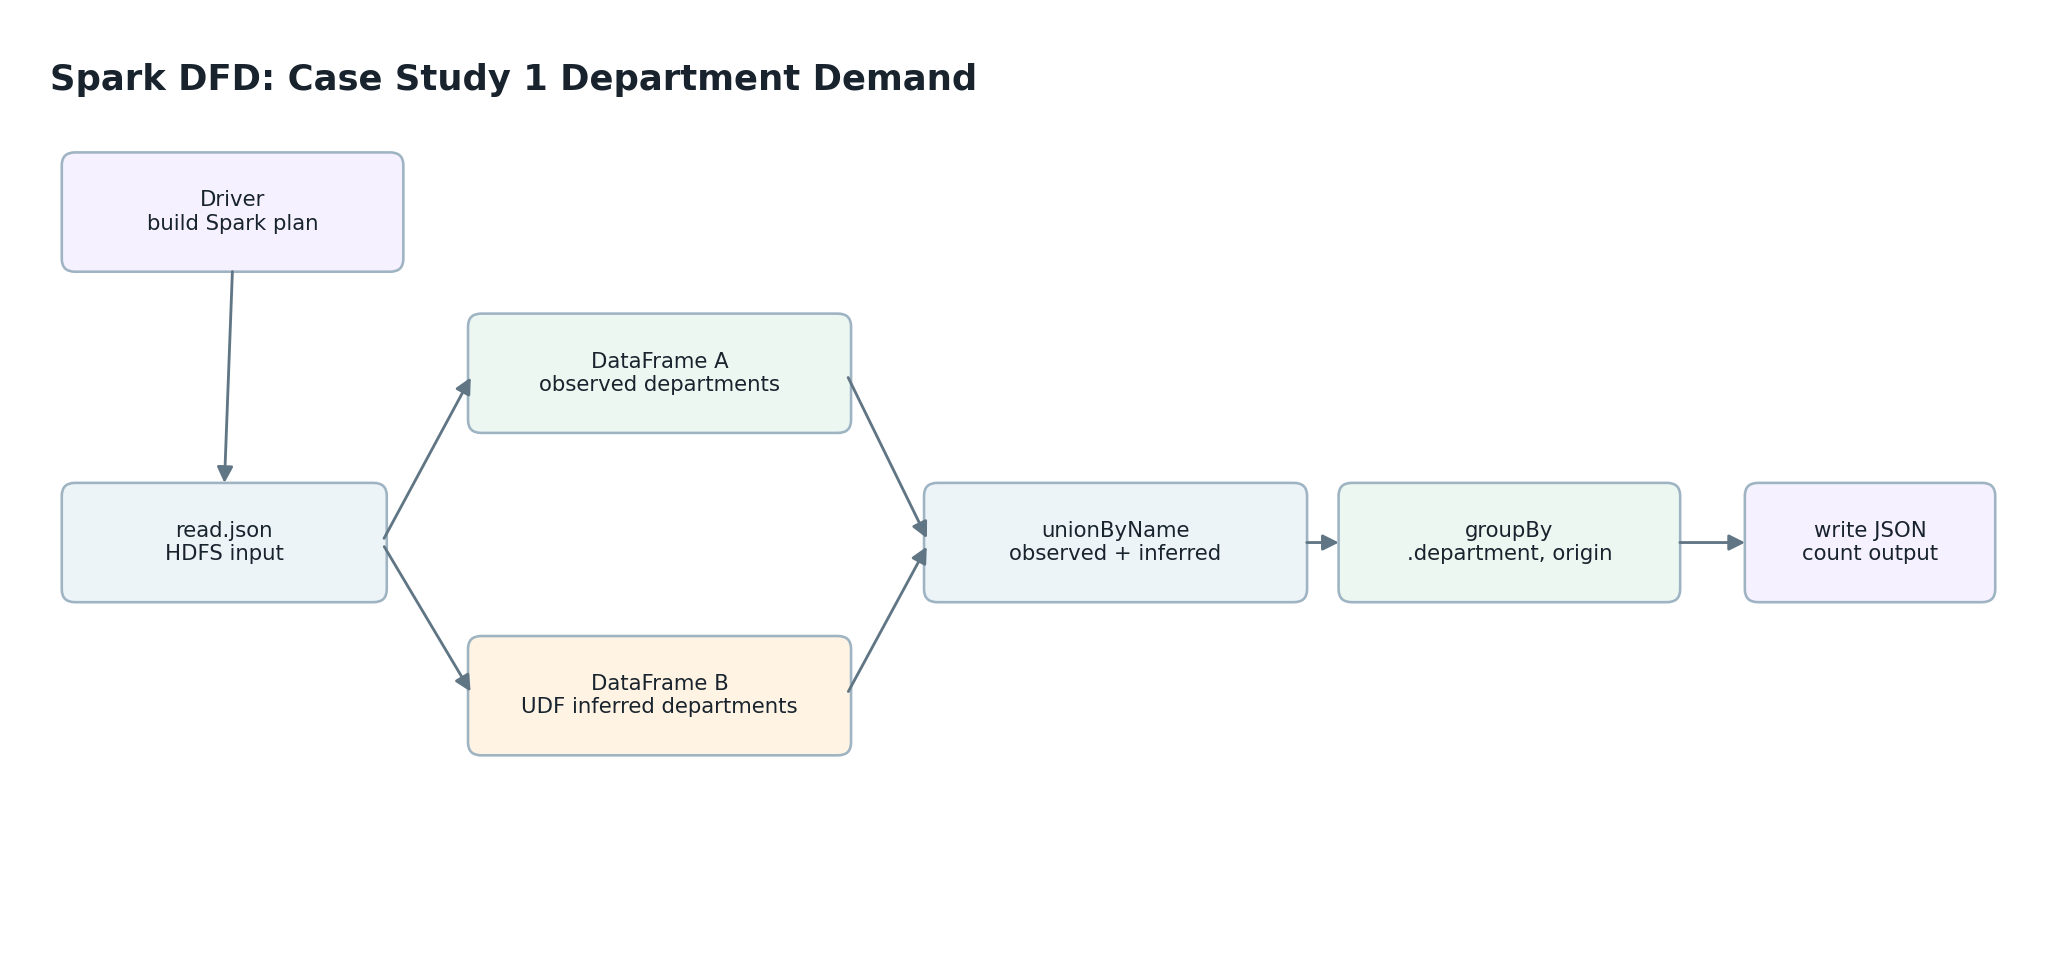
\includegraphics[width=\linewidth]{dfd_spark_case_study_1_department_demand.png}
\caption{Spark DataFrame data flow for Case Study 1: Medical Department Demand.}
\end{figure}

The Spark DFD represents the same analytical grouping without explicit key-value text lines. Spark first creates a DataFrame from the JSONL input. It then creates department rows from two paths: observed metadata rows and inferred rows. These paths are unioned into a common two-column structure, \texttt{department} and \texttt{origin}. The equivalent of the Hadoop key is therefore the DataFrame grouping expression \texttt{groupBy("department", "origin")}. The value being aggregated is an implicit row count rather than an explicit emitted integer.

\subsubsection*{Code and Output Result}

The implementation is more than a direct count over one column. Both frameworks first resolve the department field from the canonical schema, preserve whether the department was observed or inferred, and then aggregate by the compound key \texttt{(department, origin)}. The code also supports disease-to-department inference through the analytics rules file. In the final run, the rules file did not contain a disease-to-department mapping, so the 16 reported groups are observed departments from Huatuo26M-Lite. Listing~\ref{lst:cs1-code} is a condensed source excerpt from \texttt{preprocessing/common.py}, \texttt{hadoop/mapper.py}, \texttt{hadoop/reducer.py}, and \texttt{spark/healthcare\_analytics.py}.

\begin{lstlisting}[language=Python,caption={Case Study 1 source excerpts},label={lst:cs1-code}]
# Shared helper used by Hadoop when inference rules exist
def match_terms(text, terms):
    folded = text.casefold()
    return sorted({term for term in terms
                   if term and term.casefold() in folded})

# Hadoop mapper
def case_study_1(record):
    department = record.get("department") or record.get("inferred_department")
    if department:
        origin = "observed" if record.get("department") else "inferred"
        emit(["department", department, origin], 1)

def case_study_1_with_rules(record, rules):
    if record.get("department") or record.get("inferred_department"):
        case_study_1(record)
        return
    text = record.get("question", "")
    matched_diseases = match_terms(text, rules.get("diseases", []))
    departments = {
        rules.get("disease_departments", {}).get(disease)
        for disease in matched_diseases
    }
    for department in sorted(value for value in departments if value):
        emit(["department", department, "inferred"], 1)

# Hadoop reducer for count-based case studies
if is_quality_key(args.case_study, current_key):
    result = reduce_quality(accumulator)
else:
    result = {"count": accumulator}
print_result(current_key, result)

# Spark implementation
def case_study_1(df, rules):
    diseases = rules.get("diseases", [])
    disease_departments = rules.get("disease_departments", {})

    def infer_departments(question):
        folded = (question or "").casefold()
        return sorted({
            disease_departments[disease]
            for disease in diseases
            if disease.casefold() in folded and disease in disease_departments
        })

    infer_udf = F.udf(infer_departments, T.ArrayType(T.StringType()))
    observed = (
        df.where(F.coalesce("department", "inferred_department").isNotNull())
        .select(
            F.coalesce("department", "inferred_department").alias("department"),
            F.when(F.col("department").isNotNull(), "observed")
             .otherwise("inferred").alias("origin"),
        )
    )
    inferred = (
        df.where(F.coalesce("department", "inferred_department").isNull())
        .withColumn("departments", infer_udf("question"))
        .select(F.explode("departments").alias("department"))
        .withColumn("origin", F.lit("inferred"))
    )
    return (observed.unionByName(inferred)
        .groupBy("department", "origin")
        .count()
        .orderBy(F.desc("count"), "department"))
\end{lstlisting}

\begin{table}[H]
\centering
\caption{Case Study 1 output sample: highest observed department counts}
\label{tab:cs1-output}
\begin{tabular}{lr}
\toprule
Department & Count \\
\midrule
Obstetrics and Gynecology & 34,313 \\
Internal Medicine & 29,677 \\
Dermatology and Venereology & 24,668 \\
Pediatrics & 21,202 \\
ENT and Ophthalmology & 13,791 \\
\bottomrule
\end{tabular}
\end{table}

The full output contained 16 department groups in both Hadoop and Spark.

\subsection{Case Study 2: Disease and Symptom Trend Mining}

This case study identifies disease and symptom mentions in the normalized question text and, where the answer is textual, in the answer text. URL answers are not treated as medical answer text. The grouping key is term type and matched term.

\subsubsection*{Hadoop Streaming Implementation}

The Hadoop mapper builds a searchable text string from the question and any text answer. It matches disease and symptom terms from the analytics rules. Observed or inferred related disease metadata is also included as a disease term. For every matched disease or symptom, the mapper emits a term key with value 1. The Hadoop shuffle groups all equal term keys, and the reducer sums frequencies.

\begin{figure}[H]
\centering
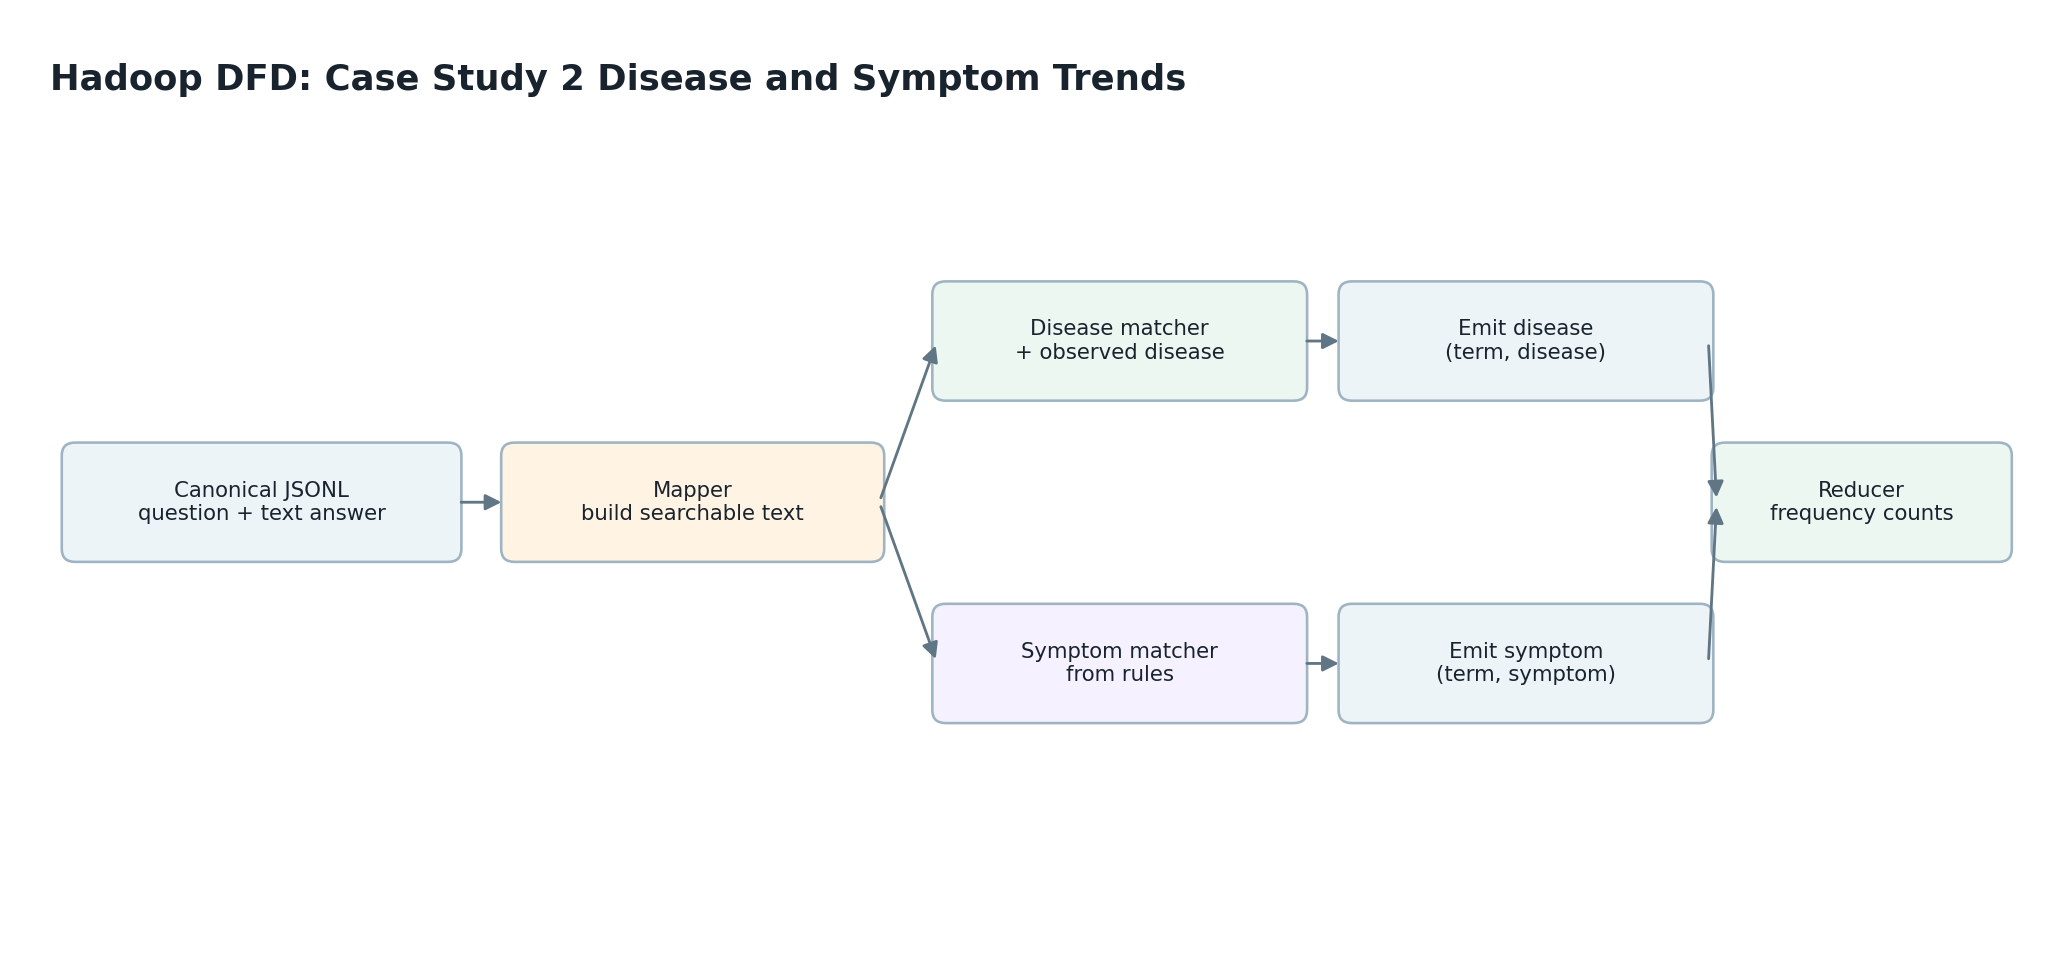
\includegraphics[width=\linewidth]{dfd_case_study_2_disease_symptom_trends.png}
\caption{Hadoop Streaming data flow for Case Study 2: Disease and Symptom Trends.}
\end{figure}

The DFD for Case Study 2 is different from Case Study 1 because one input record can produce multiple mapper outputs. A single question may mention several symptoms or diseases, so the mapper performs a one-to-many transformation. It first constructs searchable text from the normalized question and, only when \texttt{answer\_type} is \texttt{text}, the answer. URL answers are excluded from the search string because they do not contain clinical answer text. The mapper then emits one key-value pair for each matched disease or symptom. The Hadoop shuffle groups all identical medical terms, and the reducer sums the frequency of each term.

\begin{table}[H]
\centering
\caption{Case Study 2 Hadoop key-value design}
\label{tab:cs2-hadoop-kv}
\begin{tabular}{p{0.26\linewidth}p{0.62\linewidth}}
\toprule
Element & Meaning \\
\midrule
Input fields & \texttt{question}, \texttt{answer}, \texttt{answer\_type}, \texttt{related\_disease}, \texttt{inferred\_disease} \\
Mapper key & \texttt{["term", "disease", disease]} or \texttt{["term", "symptom", symptom]} \\
Mapper value & \texttt{1}, meaning one matched term occurrence in one record \\
Shuffle key & Term type plus term text; disease and symptom counts remain separate \\
Reducer output & Count for each recognized disease or symptom term \\
\bottomrule
\end{tabular}
\end{table}

\subsubsection*{Spark Implementation}

The Spark job uses user-defined functions to match diseases and symptoms from the question and text answer fields. The matched term arrays are exploded into one row per matched term. Disease rows and symptom rows are unioned, grouped by term type and term, counted, ordered by frequency, and written as JSON.

\begin{figure}[H]
\centering
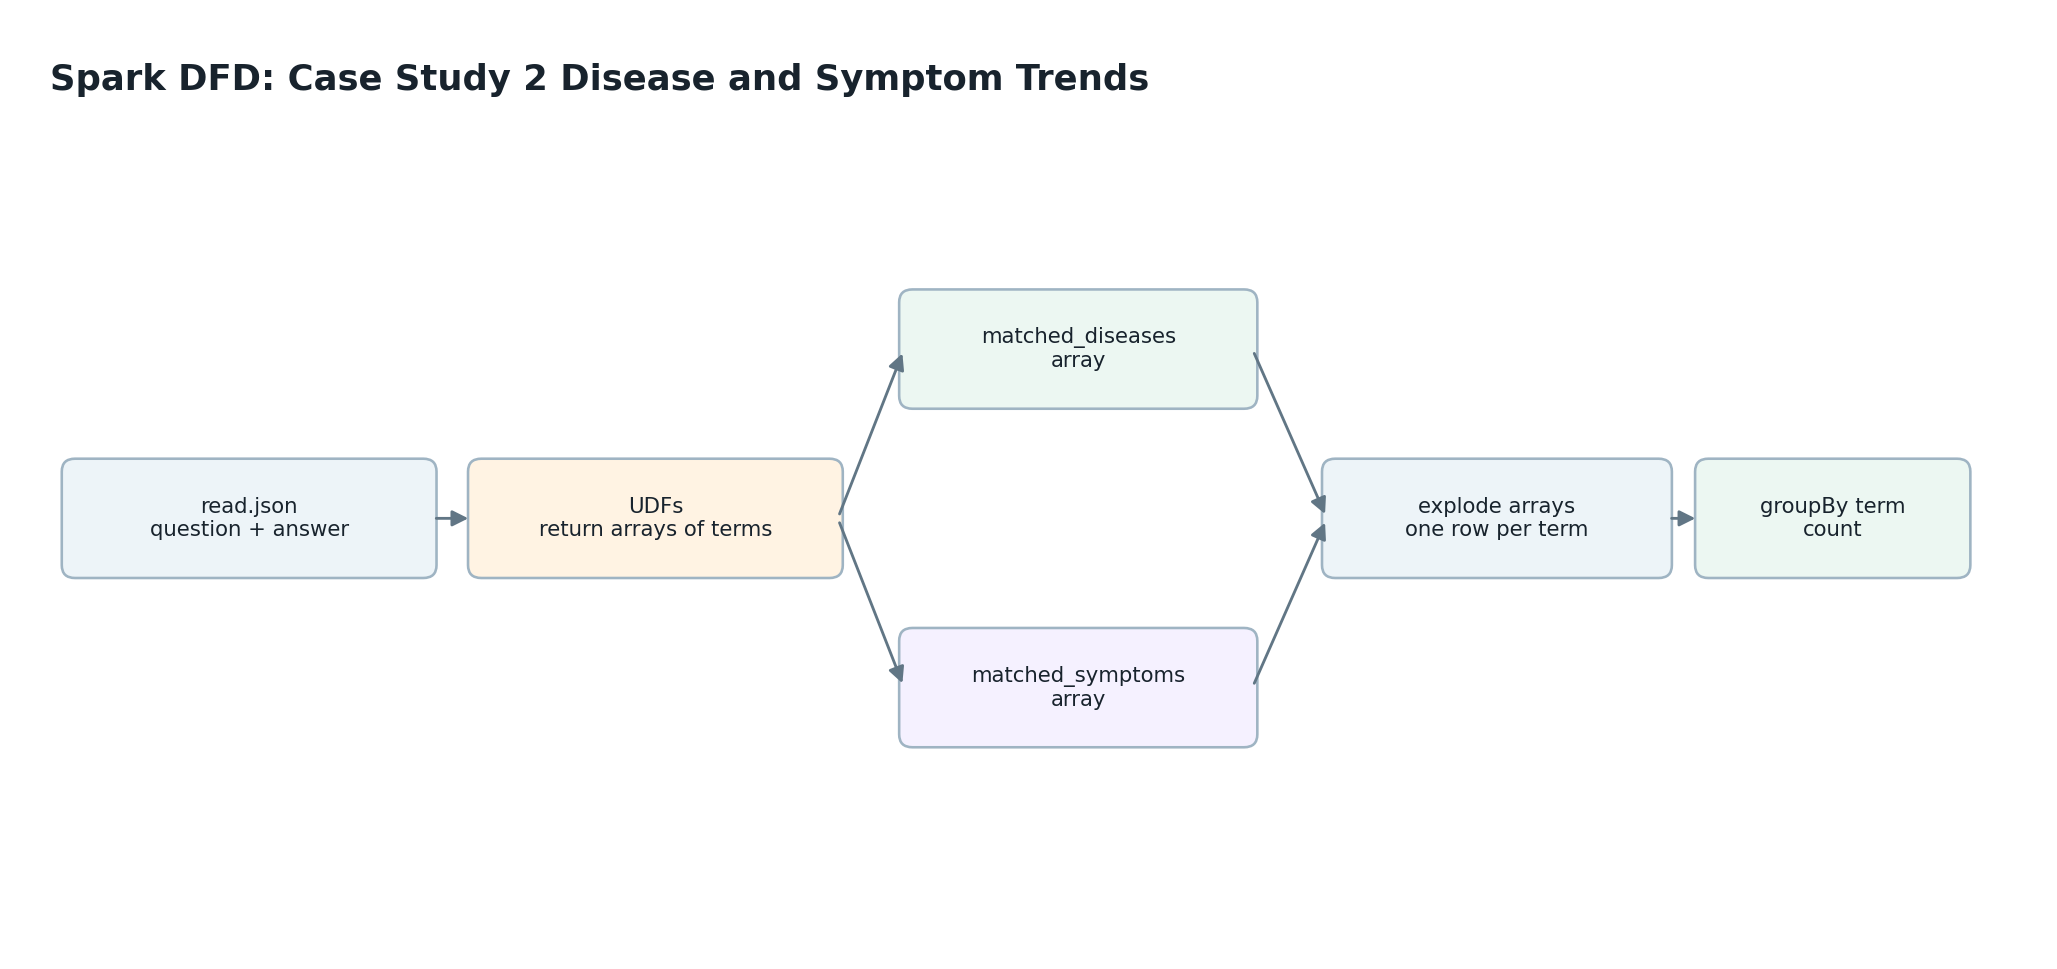
\includegraphics[width=\linewidth]{dfd_spark_case_study_2_disease_symptom_trends.png}
\caption{Spark DataFrame data flow for Case Study 2: Disease and Symptom Trends.}
\end{figure}

The Spark DFD expresses the same one-to-many transformation using arrays and \texttt{explode}. The disease UDF and symptom UDF return arrays of matched terms. \texttt{explode} converts each array element into a separate row, which is Spark's equivalent of the Hadoop mapper emitting multiple key-value pairs from one input record. After disease rows and symptom rows are unioned, the grouping key is \texttt{(term\_type, term)} and the aggregate value is the row count for that key.

\subsubsection*{Code and Output Result}

This case study uses rule-based medical term extraction, set-based duplicate control for disease matches, answer-type filtering, and an explode operation. URL answers are excluded from the searchable answer text because they are links rather than clinical answer text. Therefore, the output is a frequency table of recognized medical terms, not a count of arbitrary words. Listing~\ref{lst:cs2-code} is a condensed source excerpt from the same Hadoop, Spark, and shared-helper files used during execution.

\begin{lstlisting}[language=Python,caption={Case Study 2 source excerpts},label={lst:cs2-code}]
# Shared helper
def match_terms(text, terms):
    folded = text.casefold()
    return sorted({term for term in terms
                   if term and term.casefold() in folded})

# Hadoop mapper
def case_study_2(record, rules):
    text = record.get("question", "")
    if record.get("answer_type") == "text":
        text += " " + record.get("answer", "")

    observed_disease = (
        record.get("related_disease") or record.get("inferred_disease")
    )
    diseases = set(match_terms(text, rules.get("diseases", [])))
    if observed_disease:
        diseases.add(observed_disease)

    for disease in sorted(diseases):
        emit(["term", "disease", disease], 1)
    for symptom in match_terms(text, rules.get("symptoms", [])):
        emit(["term", "symptom", symptom], 1)

# Hadoop reducer
# The Hadoop shuffle groups equal keys before this accumulation.
accumulator += json.loads(raw_value)

# Spark implementation
def case_study_2(df, rules):
    symptom_udf = F.udf(
        lambda q, a, t: [
            term for term in rules.get("symptoms", [])
            if term.casefold() in f"{q or ''} {a if t == 'text' else ''}".casefold()
        ],
        T.ArrayType(T.StringType()),
    )
    disease_udf = F.udf(
        lambda q, a, t, observed: sorted({
            *([observed] if observed else []),
            *[
                disease for disease in rules.get("diseases", [])
                if disease.casefold()
                in f"{q or ''} {a if t == 'text' else ''}".casefold()
            ],
        }),
        T.ArrayType(T.StringType()),
    )
    diseases = (
        df.withColumn(
            "matched_diseases",
            disease_udf("question", "answer", "answer_type",
                        F.coalesce("related_disease", "inferred_disease")),
        )
        .select(F.explode("matched_diseases").alias("term"))
        .withColumn("term_type", F.lit("disease"))
    )
    symptoms = (
        df.withColumn("matched", symptom_udf("question", "answer", "answer_type"))
        .select(F.explode("matched").alias("term"))
        .withColumn("term_type", F.lit("symptom"))
    )
    return (diseases.unionByName(symptoms)
        .groupBy("term_type", "term")
        .count()
        .orderBy(F.desc("count"), "term"))
\end{lstlisting}

\begin{table}[H]
\centering
\caption{Case Study 2 output sample: most frequent disease and symptom terms}
\label{tab:cs2-output}
\begin{tabular}{llr}
\toprule
Type & Term meaning & Count \\
\midrule
Symptom & Pain & 666,529 \\
Symptom & Cough & 567,381 \\
Symptom & Fever & 471,290 \\
Symptom & Headache & 193,634 \\
Disease & Vitiligo & 3,308 \\
Disease & Common cold & 2,371 \\
\bottomrule
\end{tabular}
\end{table}

The full output contained 2,711 term groups in both Hadoop and Spark.

\subsection{Case Study 3: Medical QA Quality and Completeness}

This case study evaluates source-level quality and completeness. It measures record totals, missing questions, missing answers, URL answers, duplicate flags, question length, answer length, and quality scores where available. The grouping key is source.

\subsubsection*{Hadoop Streaming Implementation}

The Hadoop mapper emits one source-quality metrics record for every input row. The value is not just a count; it is a small metrics object containing record count, missing-value flags, URL-answer flag, duplicate flag, length sums, score count, score sum, score minimum, and score maximum. The reducer groups by source and combines these metrics. It then calculates averages, percentages, minimums, and maximums for each source.

\begin{figure}[H]
\centering
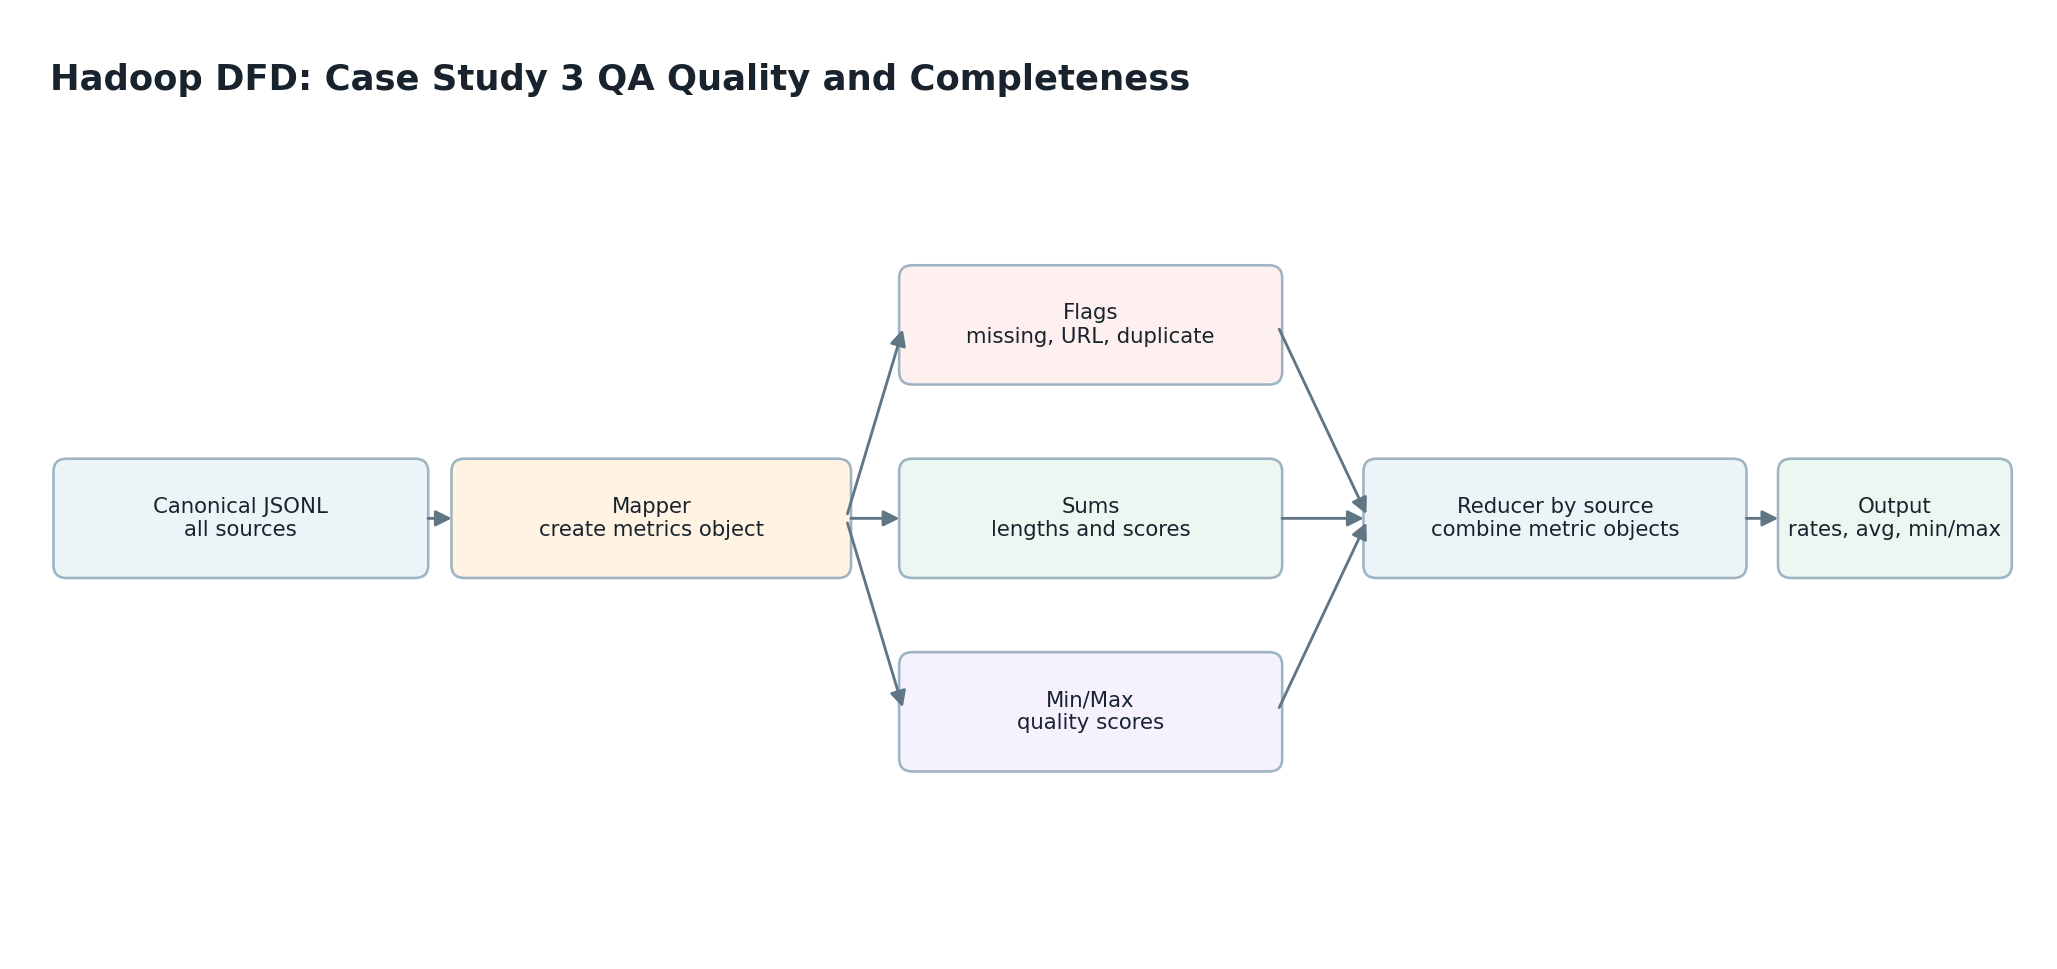
\includegraphics[width=\linewidth]{dfd_case_study_3_qa_quality.png}
\caption{Hadoop Streaming data flow for Case Study 3: Medical QA Quality and Completeness.}
\end{figure}

The Case Study 3 DFD is the most important evidence that the Hadoop job is not only a word-count style program. The mapper emits a structured metrics object instead of the integer \texttt{1}. Each value contains several partial measures for one record: completeness flags, URL-answer flag, duplicate flag, text-length sums, and quality-score components. The shuffle groups these objects by source. The reducer then performs two stages: first it adds all summable fields and maintains score minimum and maximum; then it derives averages and percentages from the accumulated totals.

\begin{table}[H]
\centering
\caption{Case Study 3 Hadoop key-value design}
\label{tab:cs3-hadoop-kv}
\begin{tabular}{p{0.26\linewidth}p{0.62\linewidth}}
\toprule
Element & Meaning \\
\midrule
Input fields & \texttt{source}, \texttt{question}, \texttt{answer\_type}, \texttt{duplicate\_flag}, \texttt{question\_length}, \texttt{answer\_length}, \texttt{quality\_score} \\
Mapper key & \texttt{["source\_quality", source]} \\
Mapper value & Metrics object with counts, flags, length sums, and score components \\
Shuffle key & Source name, so all quality metrics for one source are reduced together \\
Reducer output & Source-level records, percentages, averages, score min, and score max \\
\bottomrule
\end{tabular}
\end{table}

\subsubsection*{Spark Implementation}

The Spark job performs the same source-level analysis with DataFrame aggregations. It groups records by source, calculates counts and sums with column expressions, computes averages for question and answer length, calculates duplicate and URL-answer percentages, and derives quality-score average, minimum, and maximum. The result is written as one source-level JSON output group per source.

\begin{figure}[H]
\centering
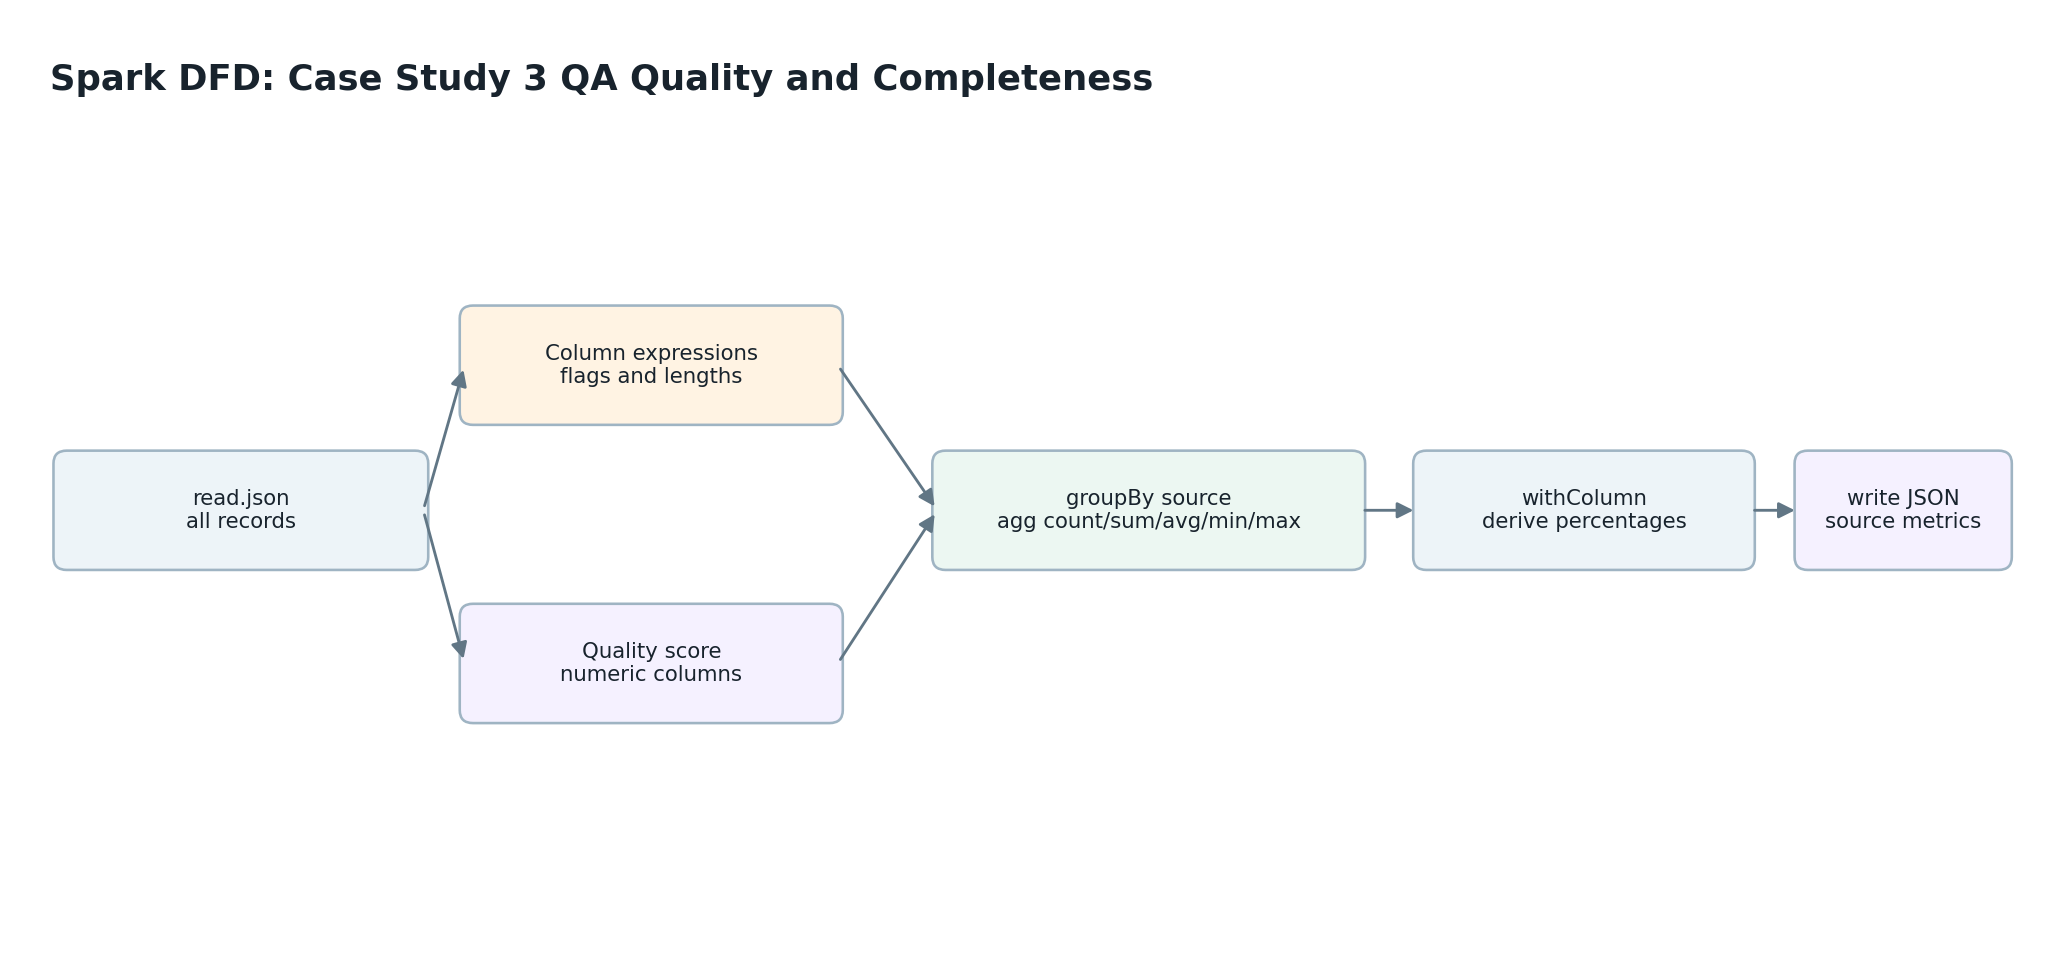
\includegraphics[width=\linewidth]{dfd_spark_case_study_3_qa_quality.png}
\caption{Spark DataFrame data flow for Case Study 3: Medical QA Quality and Completeness.}
\end{figure}

The Spark DFD replaces the explicit Hadoop metrics object with column expressions inside \texttt{agg}. The grouping key is \texttt{source}. Boolean conditions such as \texttt{answer\_type == "url"} and \texttt{duplicate\_flag} are cast or treated as numeric indicators and summed. Length and score columns are aggregated with averages, minimums, and maximums. After the grouped aggregation, Spark adds derived percentage columns. This is why the Spark flow has fewer manual reducer steps but still computes the same output measures.

\subsubsection*{Code and Output Result}

This is the strongest example that the project is not only counting words. The mapper emits a structured metrics object per record. The reducer merges numeric sums, preserves score minimum and maximum, and calculates derived quality measures after the shuffle. Spark performs the equivalent logic with grouped DataFrame aggregations and post-aggregation percentage columns. Listing~\ref{lst:cs3-code} is a condensed source excerpt from \texttt{hadoop/mapper.py}, \texttt{hadoop/reducer.py}, and \texttt{spark/healthcare\_analytics.py}.

\begin{lstlisting}[language=Python,caption={Case Study 3 source excerpts},label={lst:cs3-code}]
# Hadoop mapper
def case_study_3(record):
    score = record.get("quality_score")
    emit(["source_quality", record.get("source", "unknown")], {
        "records": 1,
        "empty_questions": int(not record.get("question")),
        "empty_answers": int(record.get("answer_type") == "empty"),
        "url_answers": int(record.get("answer_type") == "url"),
        "duplicates": int(bool(record.get("duplicate_flag"))),
        "question_length_sum": int(record.get("question_length") or 0),
        "answer_length_sum": int(record.get("answer_length") or 0),
        "score_count": int(score is not None),
        "score_sum": float(score or 0),
        "score_min": score,
        "score_max": score,
    })

# Hadoop reducer helpers
def add_quality(accumulator, value):
    for name in QUALITY_SUM_FIELDS:
        accumulator[name] += value[name]
    score_min = value["score_min"]
    score_max = value["score_max"]
    if score_min is not None:
        accumulator["score_min"] = (
            score_min if accumulator["score_min"] is None
            else min(accumulator["score_min"], score_min)
        )
    if score_max is not None:
        accumulator["score_max"] = (
            score_max if accumulator["score_max"] is None
            else max(accumulator["score_max"], score_max)
        )
    return accumulator

def reduce_quality(summed):
    records = summed["records"]
    score_count = summed["score_count"]
    return {
        **summed,
        "average_question_length": summed["question_length_sum"] / records,
        "average_answer_length": summed["answer_length_sum"] / records,
        "duplicate_percentage": 100 * summed["duplicates"] / records,
        "url_answer_percentage": 100 * summed["url_answers"] / records,
        "score_average": summed["score_sum"] / score_count if score_count else None,
        "score_min": summed["score_min"],
        "score_max": summed["score_max"],
    }

# Spark implementation
def case_study_3(df):
    score = F.col("quality_score")
    return (
        df.groupBy("source")
        .agg(
            F.count("*").alias("records"),
            F.sum(F.col("question").isNull().cast("int")).alias("empty_questions"),
            F.sum((F.col("answer_type") == "empty").cast("int")).alias("empty_answers"),
            F.sum((F.col("answer_type") == "url").cast("int")).alias("url_answers"),
            F.sum(F.col("duplicate_flag").cast("int")).alias("duplicates"),
            F.avg("question_length").alias("average_question_length"),
            F.avg("answer_length").alias("average_answer_length"),
            F.avg(score).alias("score_average"),
            F.min(score).alias("score_min"),
            F.max(score).alias("score_max"),
        )
        .withColumn("duplicate_percentage", 100 * F.col("duplicates") / F.col("records"))
        .withColumn("url_answer_percentage", 100 * F.col("url_answers") / F.col("records"))
        .orderBy("source")
    )
\end{lstlisting}

\begin{table}[H]
\centering
\caption{Case Study 3 output result: source-level quality summary}
\label{tab:cs3-output}
\begin{tabular}{lrrrr}
\toprule
Source & Records & URL answers & Duplicates & Avg. answer length \\
\midrule
Consultation & 32,708,331 & 32,708,326 & 10,025,707 & 0.000003 \\
Encyclopedia & 364,420 & 0 & 134,305 & 540.4753 \\
Knowledge Graph & 798,444 & 0 & 1,023 & 35.8706 \\
Lite & 177,703 & 0 & 1,540 & 143.8183 \\
\bottomrule
\end{tabular}
\end{table}

The full output contained four source-quality groups in both Hadoop and Spark.

\subsection{Case Study 4: Question-Type Distribution}

This case study classifies questions into intent categories such as treatment, diagnosis, symptoms, medication, prevention, cause, or other. The grouping key is question type.

\subsubsection*{Hadoop Streaming Implementation}

The Hadoop mapper applies rule-based keyword matching to the normalized question text. The first matching category is emitted as a question-type key with value 1. If no category matches, the mapper emits the other category. The Hadoop shuffle groups by question type, and the reducer sums category counts.

\begin{figure}[H]
\centering
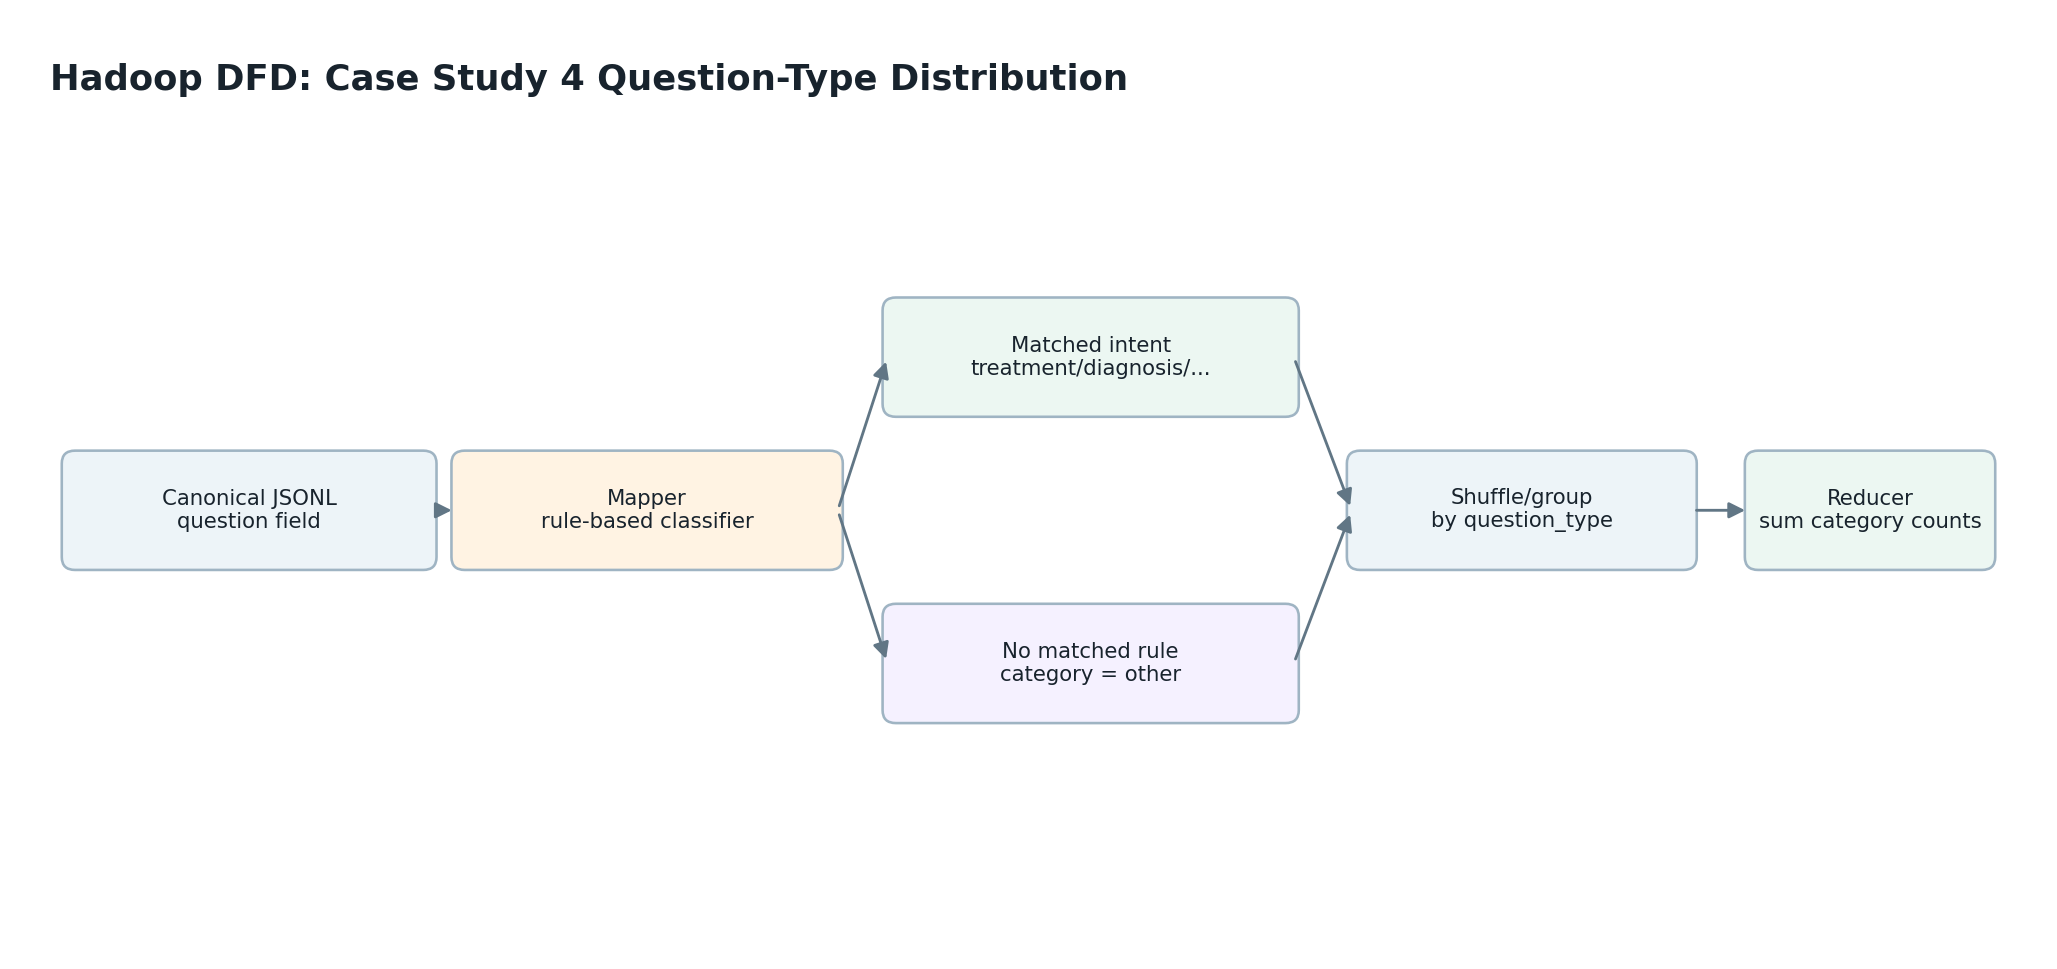
\includegraphics[width=\linewidth]{dfd_case_study_4_question_type.png}
\caption{Hadoop Streaming data flow for Case Study 4: Question-Type Distribution.}
\end{figure}

The Case Study 4 DFD shows a classification flow followed by aggregation. The mapper reads each normalized question and compares it with the configured intent keyword groups in \texttt{analytics\_rules.json}. The classifier assigns exactly one category to each question. If a question matches no rule, it is assigned to \texttt{other}. The mapper then emits the question-type key with value \texttt{1}. The shuffle groups all records with the same assigned intent category, and the reducer produces the final category distribution.

\begin{table}[H]
\centering
\caption{Case Study 4 Hadoop key-value design}
\label{tab:cs4-hadoop-kv}
\begin{tabular}{p{0.26\linewidth}p{0.62\linewidth}}
\toprule
Element & Meaning \\
\midrule
Input fields & \texttt{question} and \texttt{question\_types} rules \\
Mapper key & \texttt{["question\_type", question\_type]} \\
Mapper value & \texttt{1}, meaning one question belongs to the assigned intent category \\
Shuffle key & Question-type category, such as \texttt{treatment}, \texttt{diagnosis}, or \texttt{other} \\
Reducer output & Count for each question intent category \\
\bottomrule
\end{tabular}
\end{table}

\subsubsection*{Spark Implementation}

The Spark job applies the same rule-based classifier through a user-defined function. It creates a new \texttt{question\_type} column, groups records by that column, counts each category, orders the result, and writes the category-count output as JSON.

\begin{figure}[H]
\centering
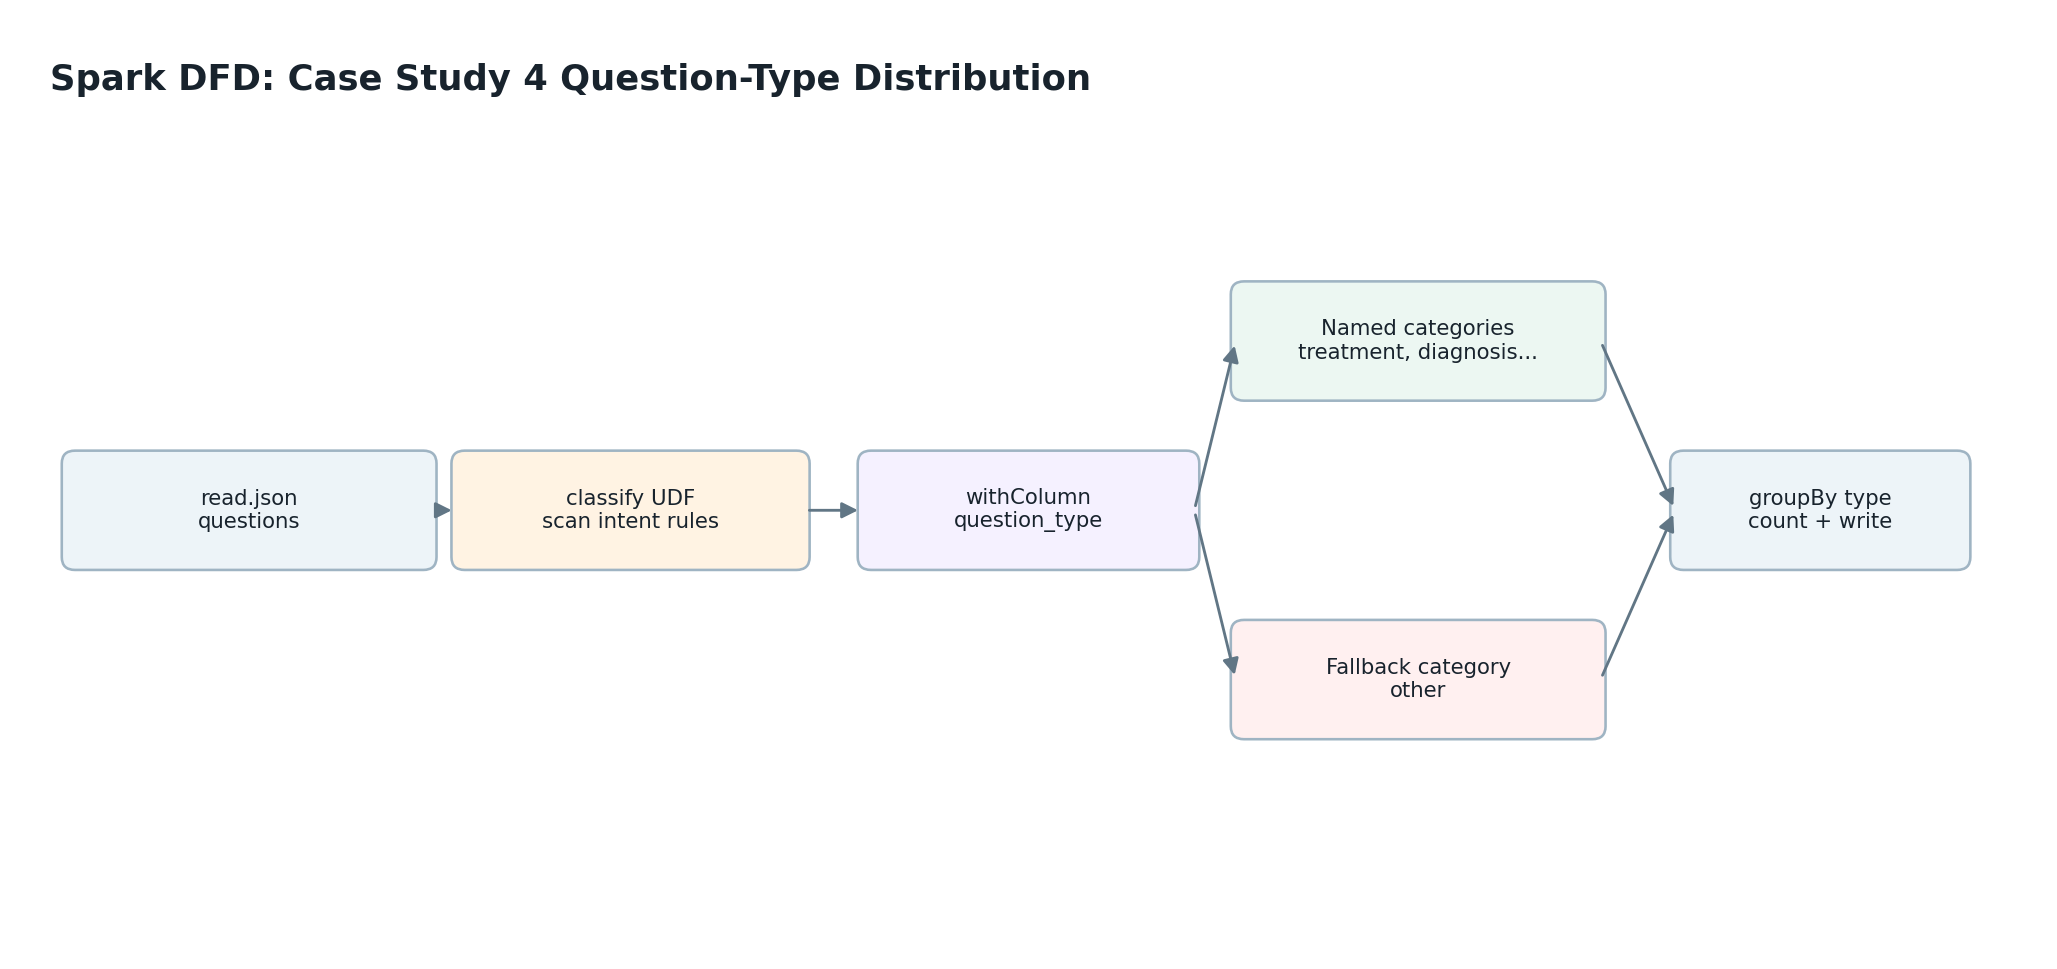
\includegraphics[width=\linewidth]{dfd_spark_case_study_4_question_type.png}
\caption{Spark DataFrame data flow for Case Study 4: Question-Type Distribution.}
\end{figure}

The Spark DFD uses the same classification rules but represents the classification result as a new DataFrame column. The UDF receives the question text and returns one category. After this transformation, the grouping key is simply \texttt{question\_type}. Spark counts rows per category and writes the distribution. Therefore, the Spark equivalent of the Hadoop emitted key \texttt{["question\_type", question\_type]} is the DataFrame column \texttt{question\_type}.

\subsubsection*{Code and Output Result}

This case study is a rule-based text classification task. The classifier scans normalized question text against medical-intent keyword groups, assigns the first matching category in deterministic sorted order, and sends unmatched records to \texttt{other}. This creates a reproducible intent distribution rather than a raw word-frequency count. Listing~\ref{lst:cs4-code} is a condensed source excerpt from \texttt{config/analytics\_rules.json}, \texttt{hadoop/mapper.py}, and \texttt{spark/healthcare\_analytics.py}.

\begin{lstlisting}[language=Python,caption={Case Study 4 source excerpts},label={lst:cs4-code}]
# Rule dictionary used by the classifier
question_types = {
    "cause": ["cause", "why", "\u539f\u56e0", "\u4e3a\u4ec0\u4e48"],
    "diagnosis": ["diagnose", "test", "\u8bca\u65ad", "\u68c0\u67e5"],
    "medication": ["medicine", "drug", "dose", "\u836f", "\u5242\u91cf"],
    "prevention": ["prevent", "avoid", "\u9884\u9632", "\u907f\u514d"],
    "symptom": ["symptom", "sign", "\u75c7\u72b6", "\u8868\u73b0"],
    "treatment": ["treat", "therapy", "cure", "\u6cbb\u7597", "\u600e\u4e48\u529e"],
}

# Hadoop mapper helpers
def classify_question(question, patterns):
    matches = [
        category
        for category, terms in sorted(patterns.items())
        if match_terms(question, terms)
    ]
    return matches[0] if matches else "other"

def case_study_4(record, rules):
    question_type = classify_question(
        record.get("question", ""), rules.get("question_types", {})
    )
    emit(["question_type", question_type], 1)

# Spark implementation
def case_study_4(df, rules):
    patterns = rules.get("question_types", {})

    def classify(question):
        folded = (question or "").casefold()
        for category in sorted(patterns):
            if any(term.casefold() in folded for term in patterns[category]):
                return category
        return "other"

    classify_udf = F.udf(classify, T.StringType())
    return (
        df.withColumn("question_type", classify_udf("question"))
        .groupBy("question_type")
        .count()
        .orderBy(F.desc("count"), "question_type")
    )
\end{lstlisting}

\begin{table}[H]
\centering
\caption{Case Study 4 output result: question-type distribution}
\label{tab:cs4-output}
\begin{tabular}{lr}
\toprule
Question type & Count \\
\midrule
Other & 24,580,705 \\
Treatment & 3,811,062 \\
Medication & 2,275,619 \\
Cause & 1,526,071 \\
Diagnosis & 1,000,666 \\
Symptom & 735,580 \\
Prevention & 119,195 \\
\bottomrule
\end{tabular}
\end{table}

The full output contained seven question-type groups in both Hadoop and Spark.

\section{Experimental Setup}

The experiment was designed to compare equivalent Hadoop Streaming and Spark implementations over the same canonical medical QA dataset. Both frameworks read the same JSONL input from HDFS and wrote JSON output groups. The full benchmark input path was:

\begin{verbatim}
/healthcare/full/input/huatuo_unified.jsonl
\end{verbatim}

Hadoop jobs used Hadoop Streaming with Python mapper and reducer programs. Spark jobs used a PySpark application submitted to YARN. Each case study was submitted separately so that execution time could be measured per analytical workload. This per-case-study layout was selected because the four case studies have different computational patterns: simple department counting, term extraction, source-level quality aggregation, and question-intent classification.

\begin{table}[H]
\centering
\caption{Experimental environment and benchmark controls}
\label{tab:experimental-setup}
\begin{tabular}{p{0.30\linewidth}p{0.60\linewidth}}
\toprule
Item & Configuration or control \\
\midrule
Execution environment & Local single-machine HDFS/YARN setup \\
Input dataset & Final canonical Huatuo JSONL dataset \\
Full input size & 34,048,898 records, about 19 GB \\
Pilot input size & 400,000 deterministic records \\
Hadoop implementation & Hadoop Streaming mapper and reducer written in Python \\
Spark implementation & PySpark DataFrame application submitted with \texttt{spark-submit} \\
Input path control & Both frameworks read the same HDFS input path \\
Output path control & Each framework wrote one output directory per case study \\
Timing method & Wall-clock elapsed time measured around each submitted job \\
Comparison unit & One case-study job per framework \\
\bottomrule
\end{tabular}
\end{table}

The benchmark does not claim to represent a production multi-node cluster. Its purpose is to evaluate the two frameworks fairly within the same local HDFS/YARN environment. The same input data, same case-study definitions, and same output-group checks were used for both implementations.

\section{Results and Analysis}

\subsection{Pilot Benchmark}

The pilot benchmark used the deterministic 400,000-record subset described earlier. Its main purpose was validation: confirm that the Hadoop and Spark jobs could read the canonical schema, run the four case studies, write outputs, and produce matching output-group counts before the full dataset was processed.

\begin{figure}[H]
\centering

\includegraphics[width=0.95\linewidth]{pilot_execution_time.png}
\caption{Pilot HDFS/YARN execution time by case study.}
\end{figure}

\begin{table}[H]
\centering
\caption{Pilot HDFS/YARN benchmark results}
\label{tab:pilot-results-final}
\begin{tabular}{lrrr}
\toprule
Case study & Output groups & Hadoop & Spark \\
\midrule
Department demand & 16 & 18.763 s & 29.630 s \\
Disease and symptom trends & 2,301 & 18.558 s & 31.256 s \\
QA quality and completeness & 4 & 19.602 s & 25.309 s \\
Question-type distribution & 7 & 18.560 s & 23.310 s \\
\midrule
Total & 2,328 & 75.483 s & 109.505 s \\
\bottomrule
\end{tabular}
\end{table}

The pilot results show that Hadoop Streaming was faster on the smaller dataset. This was expected because Spark pays startup, scheduling, DataFrame planning, and Python UDF overhead before the workload is large enough to amortize those costs. The pilot therefore should be interpreted as a readiness and correctness benchmark, not as the final framework conclusion.

\subsection{Full Dataset Benchmark}

The full benchmark used the 34,048,898-record canonical dataset in HDFS. Spark completed three of the four case studies faster, while Hadoop Streaming was slightly faster for disease and symptom trend mining.

\begin{figure}[H]
\centering

\includegraphics[width=0.95\linewidth]{full_execution_time.png}
\caption{Full HDFS/YARN execution time by case study.}
\end{figure}

\begin{table}[H]
\centering
\caption{Full HDFS/YARN benchmark results}
\label{tab:full-benchmark}
\begin{tabular}{lrrr}
\toprule
Case study & Output groups & Hadoop & Spark \\
\midrule
Department demand & 16 & 128.071 s & 117.327 s \\
Disease and symptom trends & 2,711 & 139.457 s & 149.503 s \\
QA quality and completeness & 4 & 273.549 s & 82.296 s \\
Question-type distribution & 7 & 204.027 s & 113.497 s \\
\bottomrule
\end{tabular}
\end{table}

\begin{figure}[H]
\centering
\begin{subfigure}{0.47\linewidth}
\centering
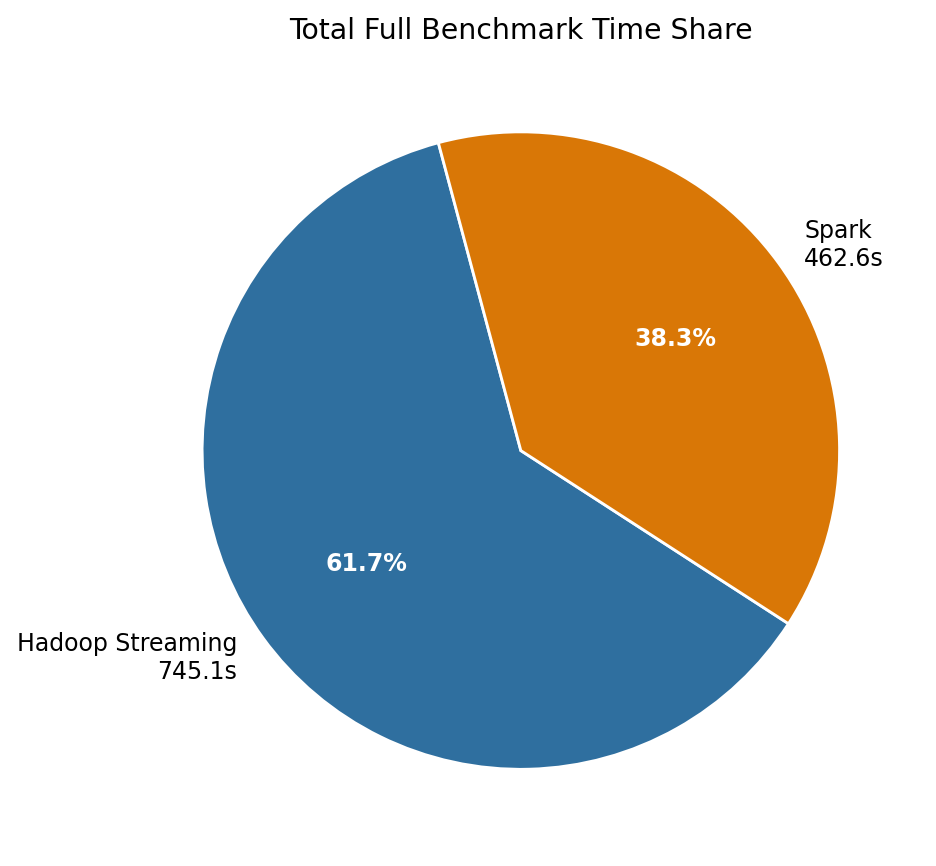
\includegraphics[width=\linewidth]{full_total_time_share.png}
\caption{Total time share}
\end{subfigure}
\hfill
\begin{subfigure}{0.47\linewidth}
\centering
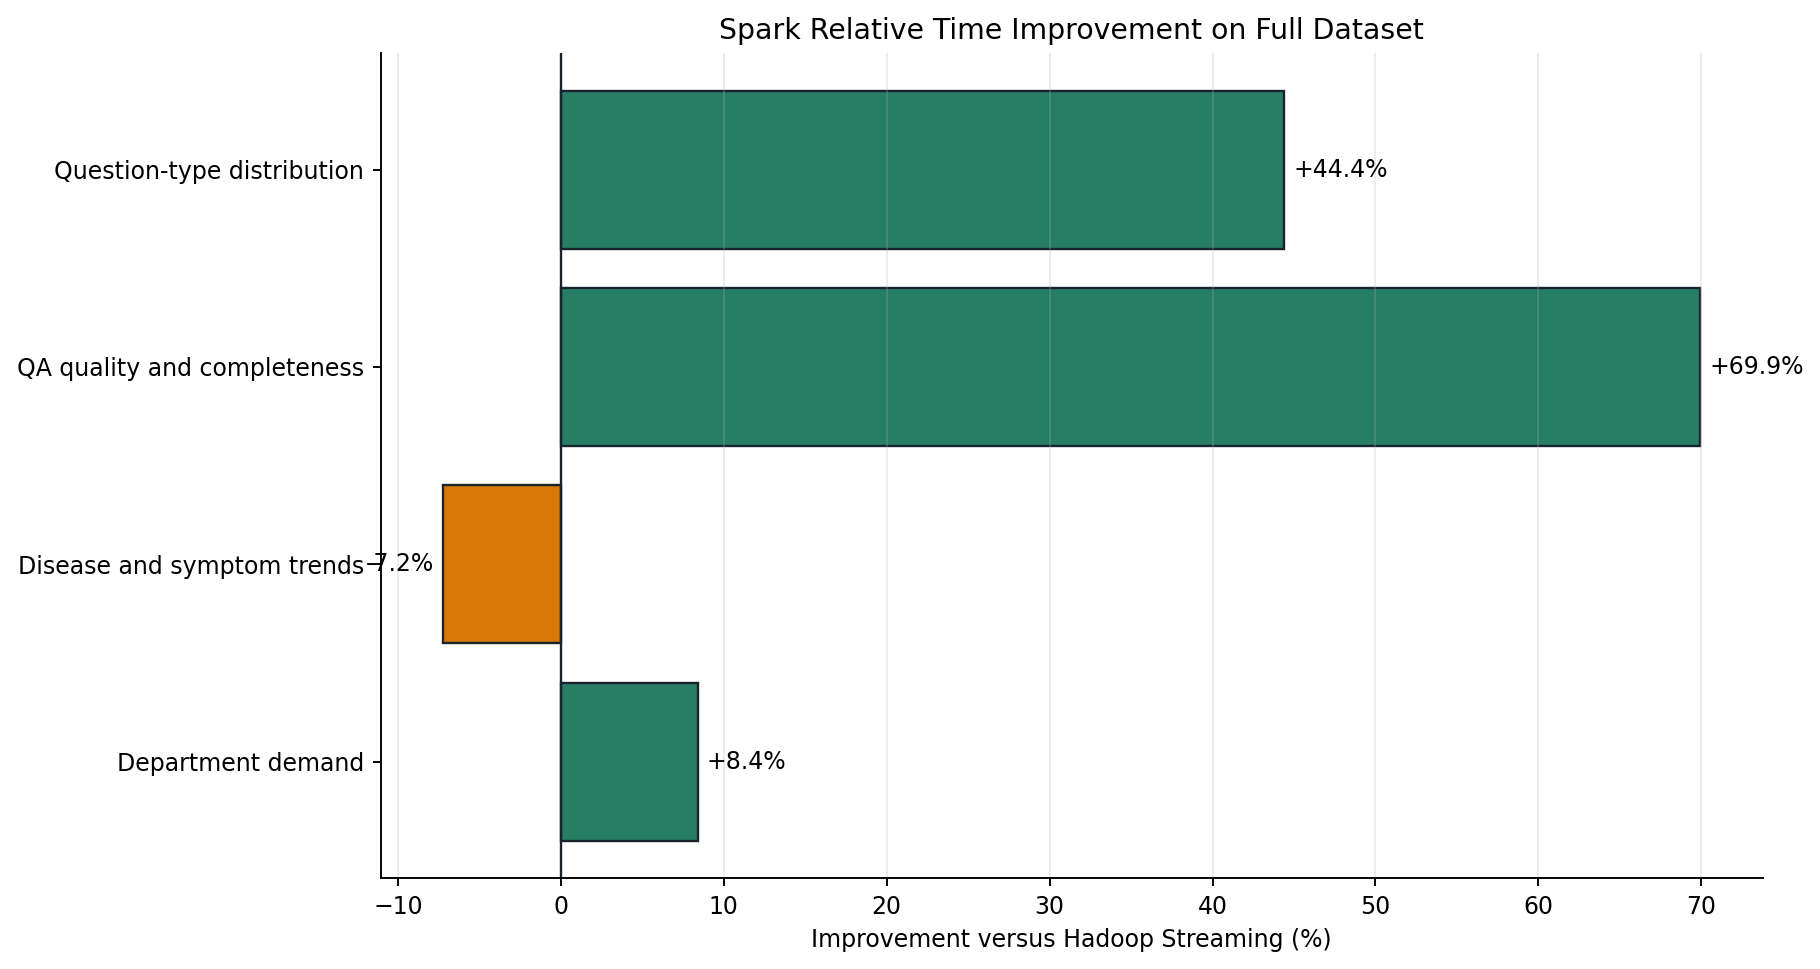
\includegraphics[width=\linewidth]{full_spark_speedup.png}
\caption{Spark relative improvement}
\end{subfigure}
\caption{Full benchmark summary charts. Positive improvement means Spark was faster than Hadoop Streaming.}
\end{figure}

\begin{figure}[H]
\centering
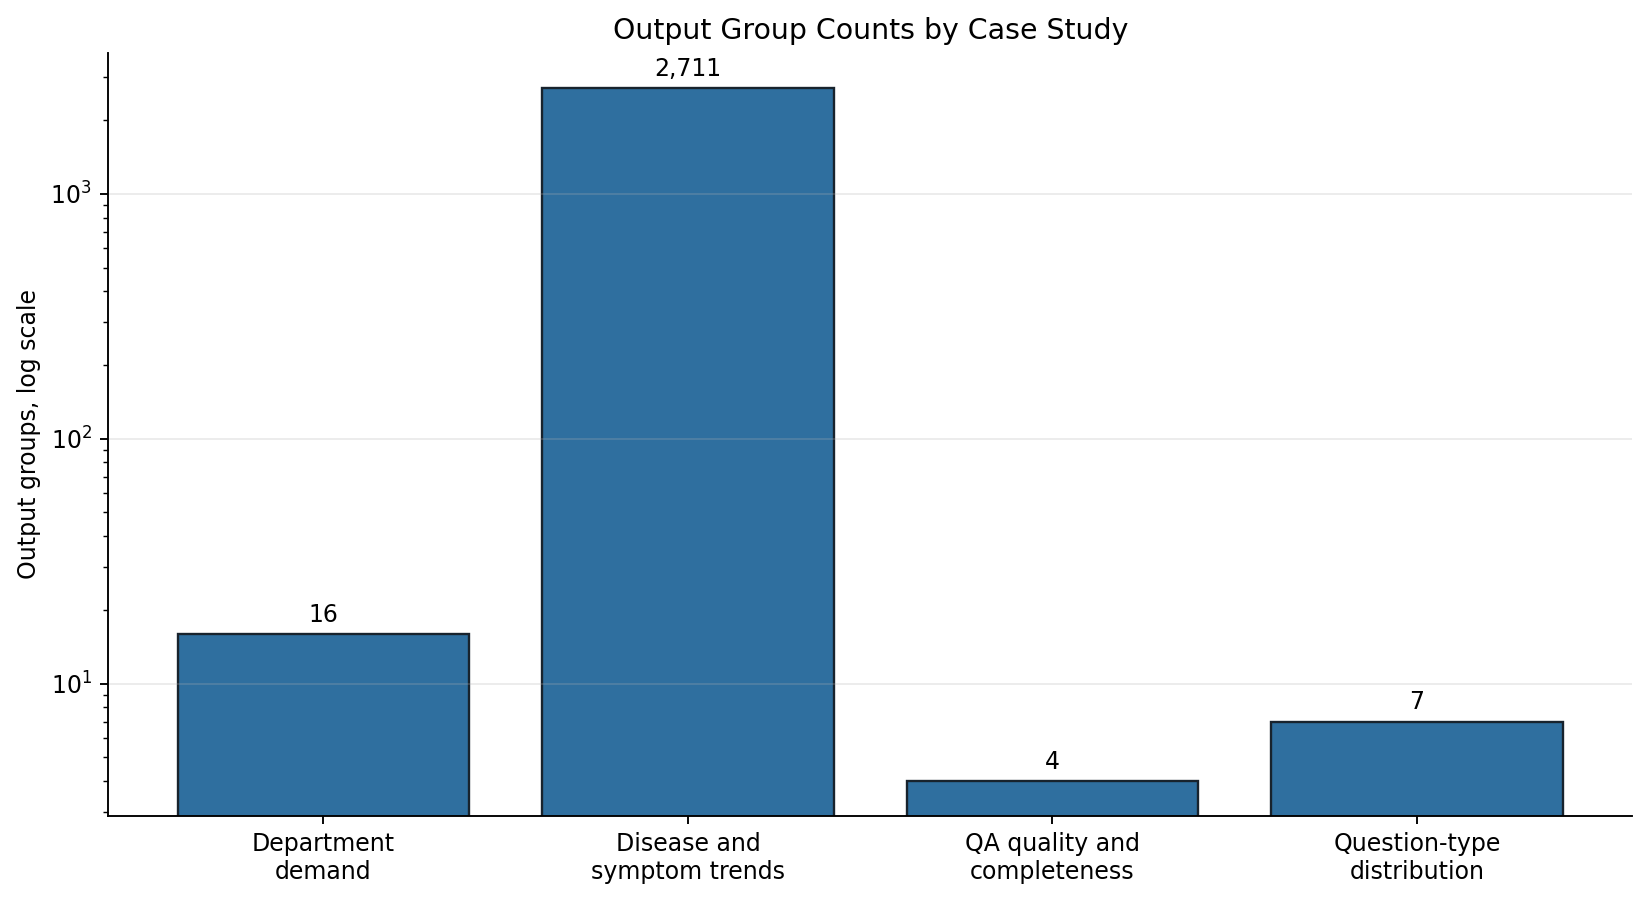
\includegraphics[width=0.82\linewidth]{full_output_groups.png}
\caption{Output group counts by case study. A logarithmic scale is used because disease and symptom trends produced many more groups than the other case studies.}
\end{figure}

\begin{table}[H]
\centering
\caption{Full benchmark interpretation by case study}
\label{tab:full-interpretation}
\begin{tabular}{p{0.29\linewidth}rrp{0.25\linewidth}}
\toprule
Case study & Faster framework & Difference & Interpretation \\
\midrule
Department demand & Spark & 10.744 s & Spark was slightly faster for department grouping. \\
Disease and symptom trends & Hadoop & 10.046 s & Hadoop was slightly faster for streaming text matching. \\
QA quality and completeness & Spark & 191.253 s & Spark was much faster for source-level metric aggregation. \\
Question-type distribution & Spark & 90.530 s & Spark was faster despite UDF classification overhead. \\
\bottomrule
\end{tabular}
\end{table}

Across the four full case studies, Hadoop Streaming required 745.104 seconds in total, while Spark required 462.623 seconds. Spark therefore reduced total measured execution time by approximately 37.9\% compared with Hadoop Streaming in the full benchmark. The most important change from the pilot is that the larger dataset made Spark's fixed overhead less dominant, allowing its aggregation execution model to become more beneficial.

\section{Discussion}

The results show that framework performance depends on workload shape, not only dataset size. The pilot benchmark made Hadoop appear faster because Spark startup and planning overhead were large relative to the small input size. The full dataset provides a more meaningful comparison because the fixed startup cost becomes smaller relative to the total workload. Once the complete 34-million-record dataset was used, Spark became faster in three of the four case studies.

Hadoop Streaming remained competitive for disease and symptom trend mining. That case study is close to a sequential text scan: read a record, search for configured disease and symptom terms, emit matched terms, and count frequencies. Hadoop Streaming handles this style of key-value processing naturally, and its overhead is relatively small.

Spark performed especially well for QA quality and completeness. That case study computes multiple metrics at source level, including counts, percentages, averages, minimums, and maximums. Spark's DataFrame aggregation model is well suited to this type of operation because the query plan can combine multiple aggregations in one grouped computation. The result was the largest performance difference in the full benchmark.

The department demand and question-type distribution results also support this interpretation. Department demand is a small grouped aggregation, so Spark was only slightly faster. Question-type distribution requires rule-based classification, but the final aggregation has only seven categories. Spark still performed better on the full dataset because the larger input size made startup overhead less important than scan and aggregation efficiency.

Analytically, the case studies are not simply word counting. They combine schema normalization, provenance preservation, answer-type classification, missing-value checks, duplicate hashing, rule-based term extraction, metadata grouping, quality-score aggregation, length aggregation, and framework-level performance evaluation. Counting is only the final aggregation operation after the dataset has been transformed into meaningful analytical keys and metrics.

\section{Limitations}

This project has several limitations. First, the experiments were executed in a local single-machine HDFS/YARN environment rather than a production multi-node cluster. The results are valid for the controlled environment used in the project, but they should not be generalized as universal Hadoop-versus-Spark performance claims.

Second, the benchmark used one measured run per case study in the final report. Repeated runs with warm-up, confidence intervals, and controlled resource monitoring would make the performance comparison stronger. The current results are still useful because both frameworks used the same input, same machine, same local cluster services, and equivalent case-study logic.

Third, disease, symptom, and question-type detection were rule-based. This is appropriate for transparent MapReduce-style analytics, but it is not equivalent to clinical natural language understanding. A future version could compare rule-based extraction with Chinese medical NLP models, named entity recognition, or embedding-based classification.

Fourth, the analysis depends on available dataset fields. Consultation QA answers are mostly URLs, which limits answer-text analysis for that source. The report handles this by explicitly classifying URL answers and avoiding direct URL-length interpretation as answer content.

Finally, duplicate detection used normalized question hashes. This identifies exact normalized question repetition, but it does not detect semantic duplicates where two differently worded questions ask the same thing. Semantic deduplication is left for future work.

\section{Conclusion}

This project successfully transformed four heterogeneous Huatuo medical QA sources into a single canonical analytical dataset and used it to execute four equivalent Hadoop Streaming and Apache Spark case studies. The final dataset contained 34,048,898 records, occupied about 19 GB, preserved source provenance, classified answer types, exposed duplicate questions, and included derived fields needed for distributed analytics.

The project followed the complete big-data analytics lifecycle: data acquisition, aggregation, preprocessing, integration, cleaning, reduction through a deterministic pilot, transformation into canonical JSONL, distributed analysis, evaluation, and reporting. The pilot stage confirmed correctness and readiness, while the full HDFS/YARN benchmark provided the main performance evidence.

The final benchmark showed that Spark was faster in three of the four case studies and reduced total measured execution time by approximately 37.9\% compared with Hadoop Streaming. Hadoop remained competitive for the disease and symptom trend case study, where the workload resembled a sequential text scan with key-value counting. These findings show that Hadoop Streaming is effective for simple streaming aggregation, while Spark becomes more advantageous for larger and more aggregation-heavy analytical workloads.

Overall, the project demonstrates how heterogeneous healthcare QA data can be standardized, validated, analyzed, and benchmarked using big-data processing frameworks. The final report, figures, data-flow diagrams, and benchmark tables provide a reproducible explanation of both the technical pipeline and the analytical results.

\bibliographystyle{unsrt}
\bibliography{references}

\end{document}
